\section{Visualization}\label{subsec::dual_vis}

% Figure~\ref{fig::result_mnist_edge_vis} illustrates additional visualization results for the digit generation experiments. Figure~\ref{fig::result_blondhair1}, Figure~\ref{fig::result_blondhair2}, and Figure~\ref{fig::result_blondhair3} present additional visualization results of the generation of faces with the blond-hair attribute and without the blond-hair attribute. Figure~\ref{fig::result_smiling1}, Figure~\ref{fig::result_smiling2}, and Figure~\ref{fig::result_smiling3} present additional visualization results of the generation of faces with the smiling attribute and without the smiling attribute. Figure~\ref{fig::result_eyeglass1}, Figure~\ref{fig::result_eyeglass2}, and Figure~\ref{fig::result_eyeglass3} present additional visualization results of the generation of faces with the eyeglasses attribute and without the eyeglasses attribute. Figure~\ref{fig::result_rgbd1}, Figure~\ref{fig::result_rgbd2}, Figure~\ref{fig::result_nyu1}, and  Figure~\ref{fig::result_nyu2} present additional visualization results of the generation of RGB and depth image experiments. 

\begin{figure}[tbh!]
\centering
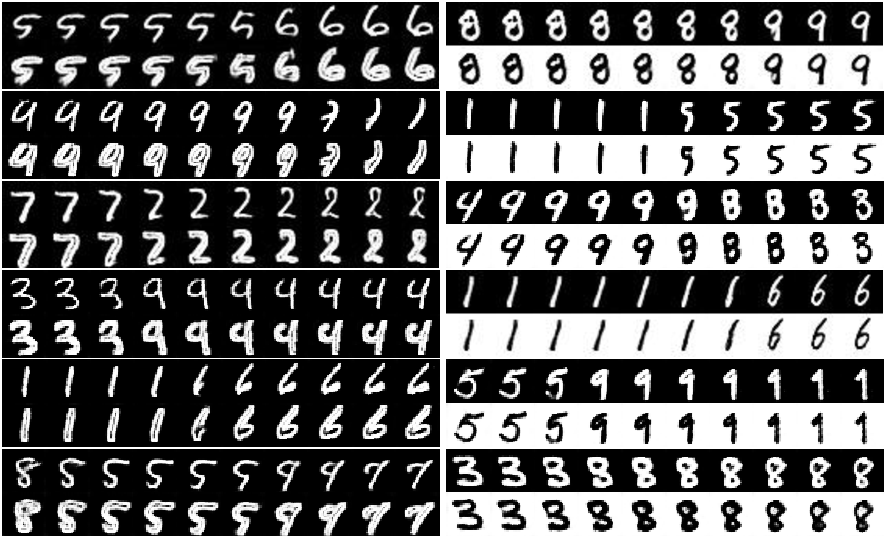
\includegraphics[trim=0.0in 0.0in 0.0in 0in, width=1.0\textwidth]{result_mnist.pdf}
\caption{Left: generation of digit and corresponding edge images. Right: generation of digit and corresponding negative images. We visualized the CoGAN results by rendering pairs of images, using the vectors that corresponded to paths connecting two pints in the input noise space. For each of the sub-figures, the top row was from $\text{GAN}_1$ and the bottom row was from $\text{GAN}_2$. Each of the top and bottom pairs was rendered using the same input noise vector. We observed that for both tasks the CoGAN learned to synthesized corresponding images in the two domains. This was interesting because there were no corresponding images in the training datasets. The correspondences were figured out during training in an unsupervised fashion.}
\label{fig::result_mnist_edge_vis}
\end{figure}

\begin{figure*}[thb!]
\centering
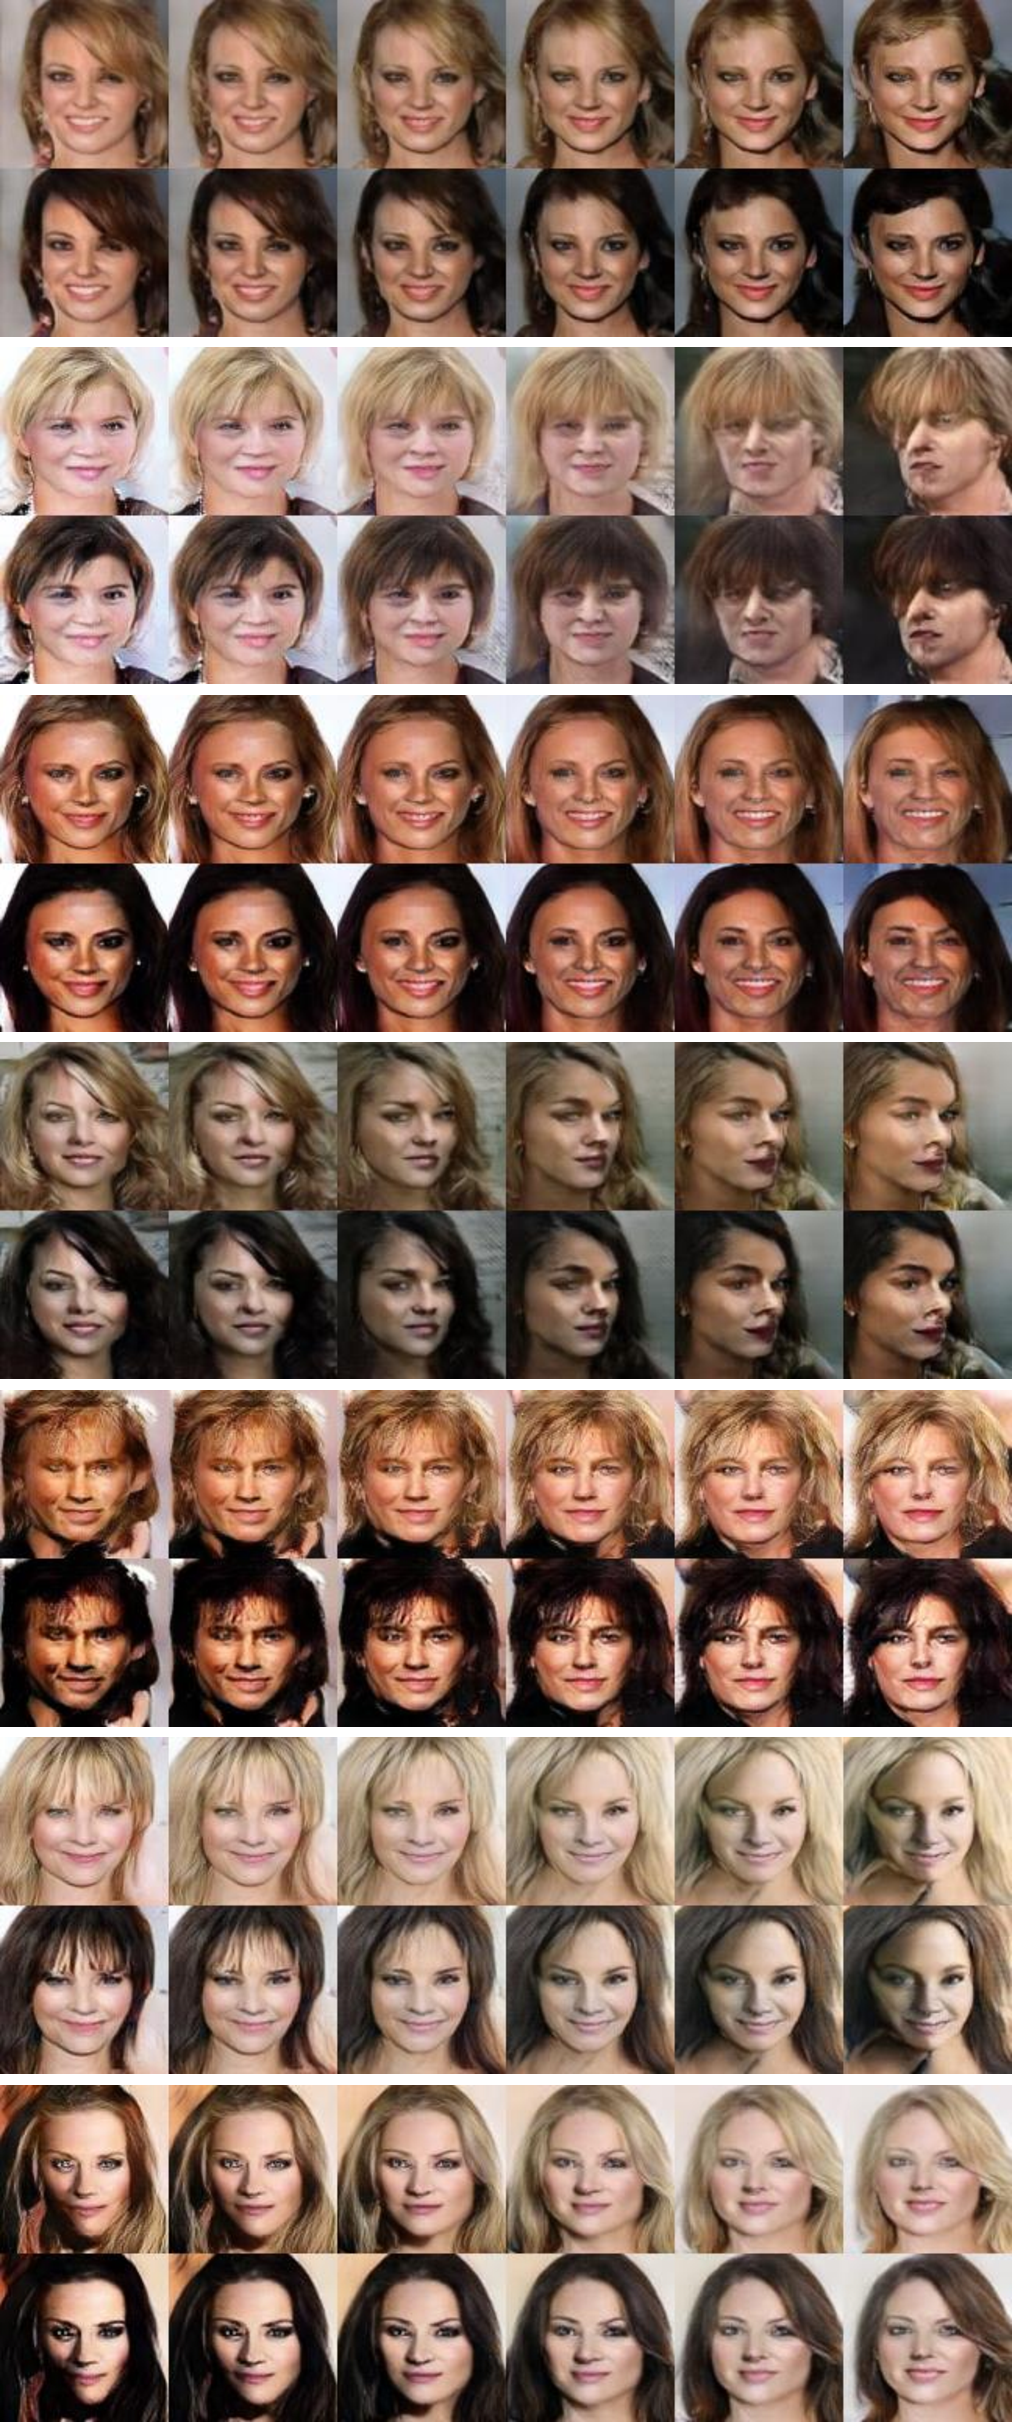
\includegraphics[trim=0in 0in 0in 0in, width=0.65\textwidth]{result_face_blondhair_big1.pdf}
\caption{Generation of faces with blond hair and without blond hair.}
\label{fig::result_blondhair1}
\end{figure*}
\begin{figure*}[thb!]
\centering
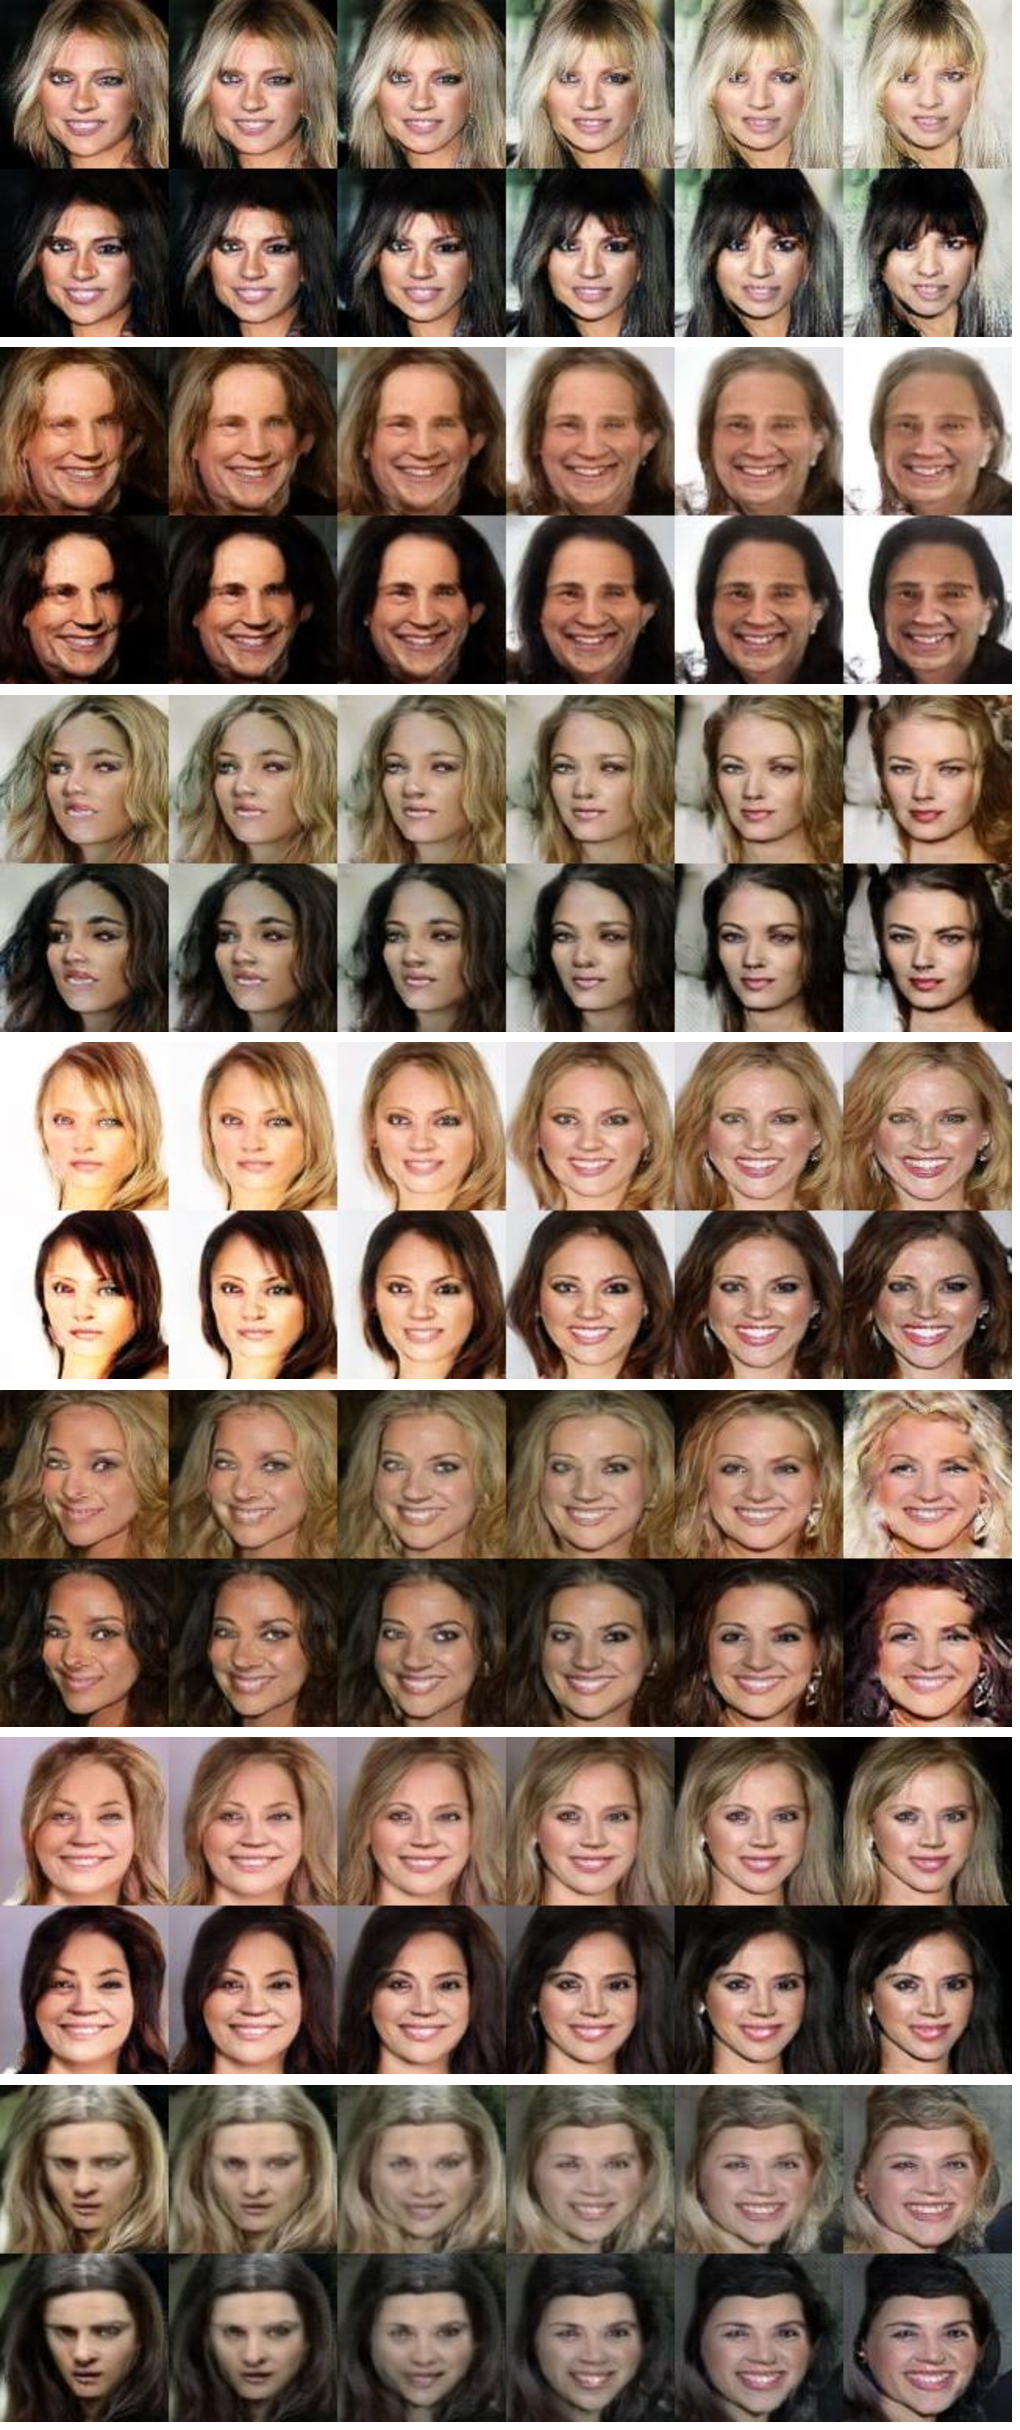
\includegraphics[trim=0in 0in 0in 0in, width=0.65\textwidth]{result_face_blondhair_big2.pdf}
\caption{Generation of faces with blond hair and without blond hair.}
\label{fig::result_blondhair2}
\end{figure*}
\begin{figure*}[thb!]
\centering
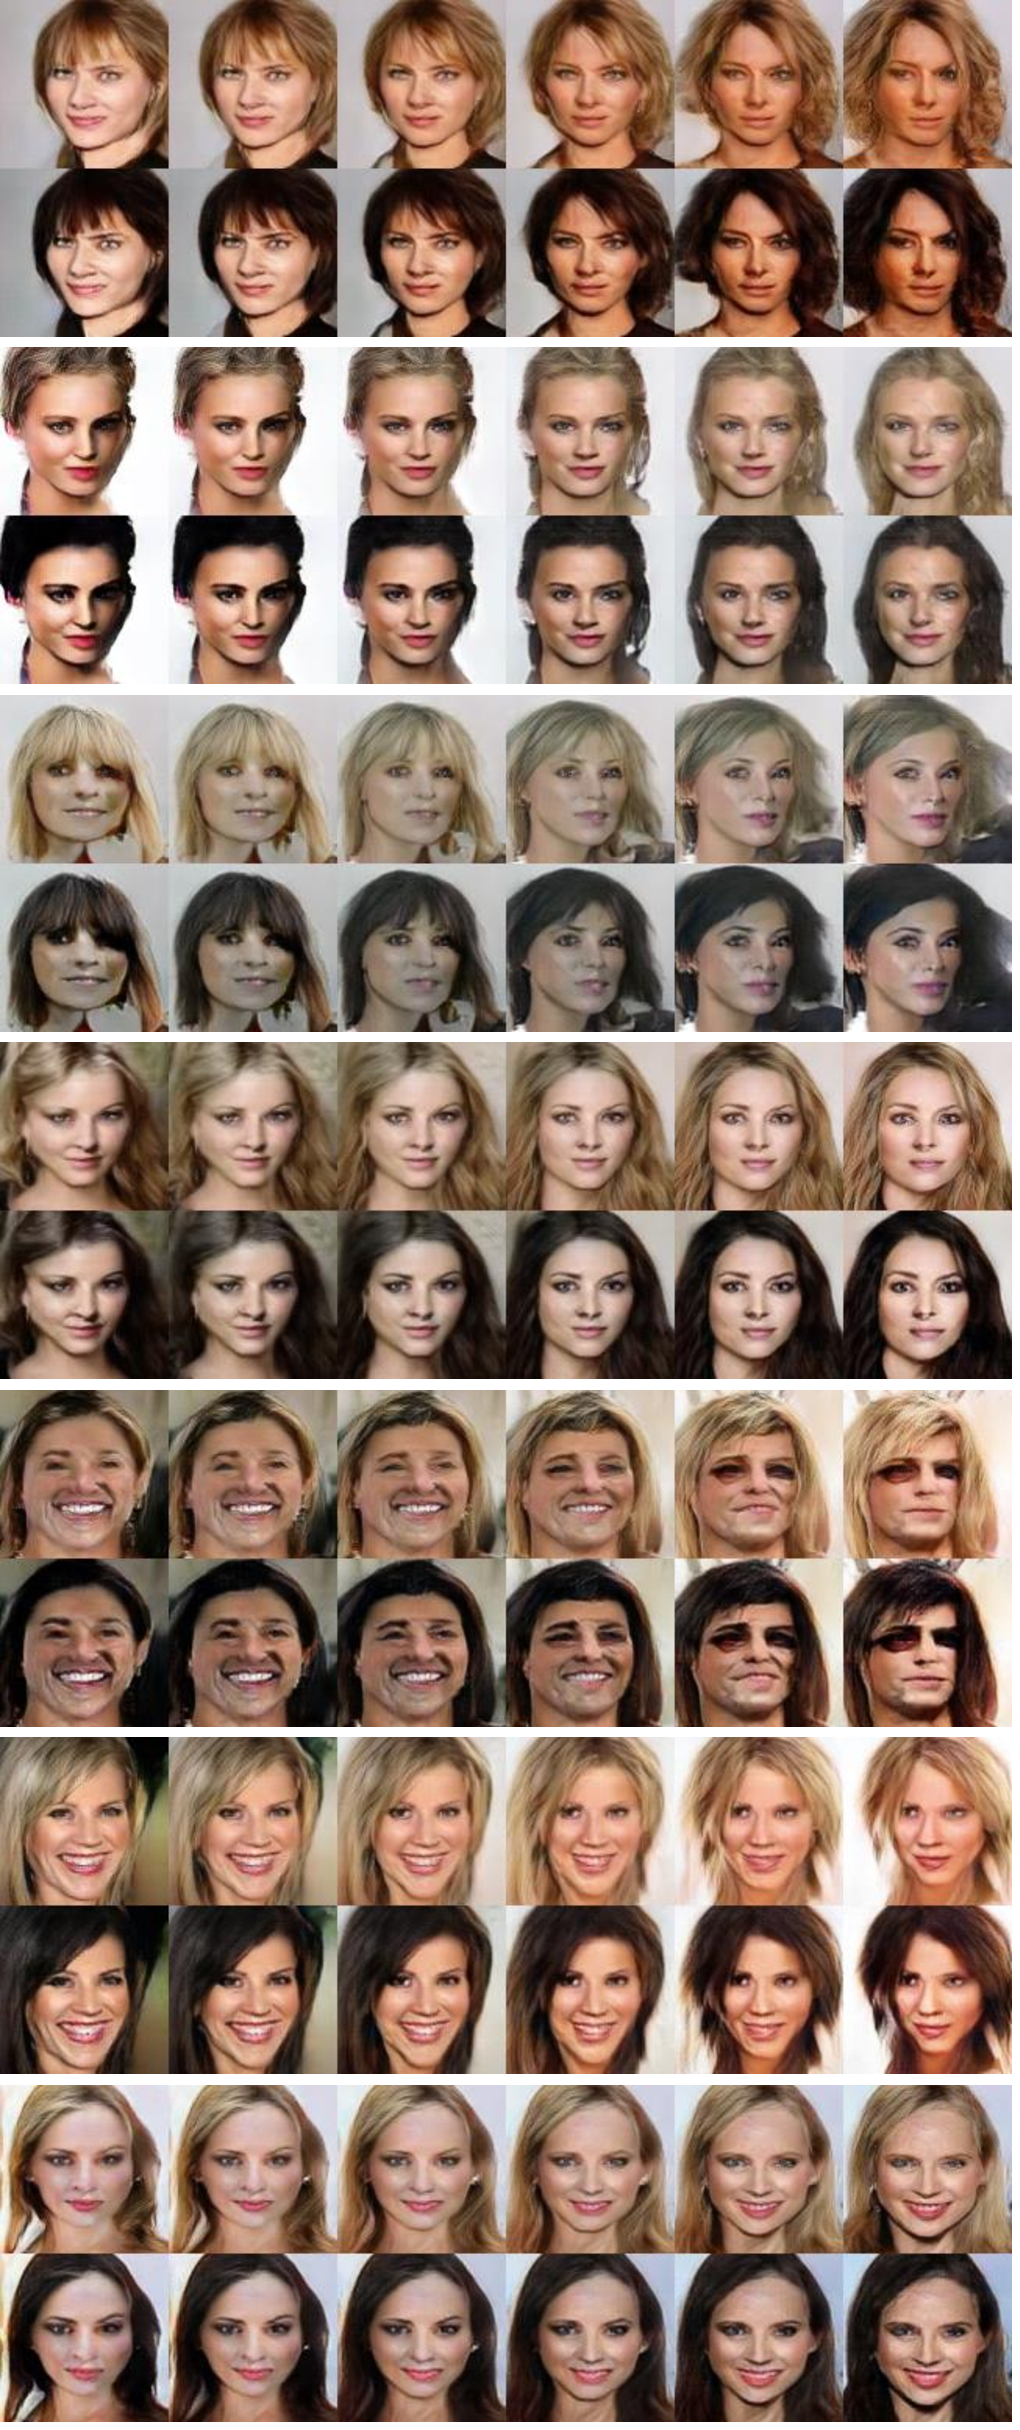
\includegraphics[trim=0in 0in 0in 0in, width=0.65\textwidth]{result_face_blondhair_big3.pdf}
\caption{Generation of faces with blond hair and without blond hair.}
\label{fig::result_blondhair3}
\end{figure*}
% %%%%%%%%%%%%%%%%%%%%%%%%%%%%%%%%%%%%%%%%%%%%%%%%%%%%%%%%%%%%%%%%%%%%%%%%%%%%%%%%%%%%%%%%%%%%%%%%%%
\begin{figure*}[thb!]
\centering
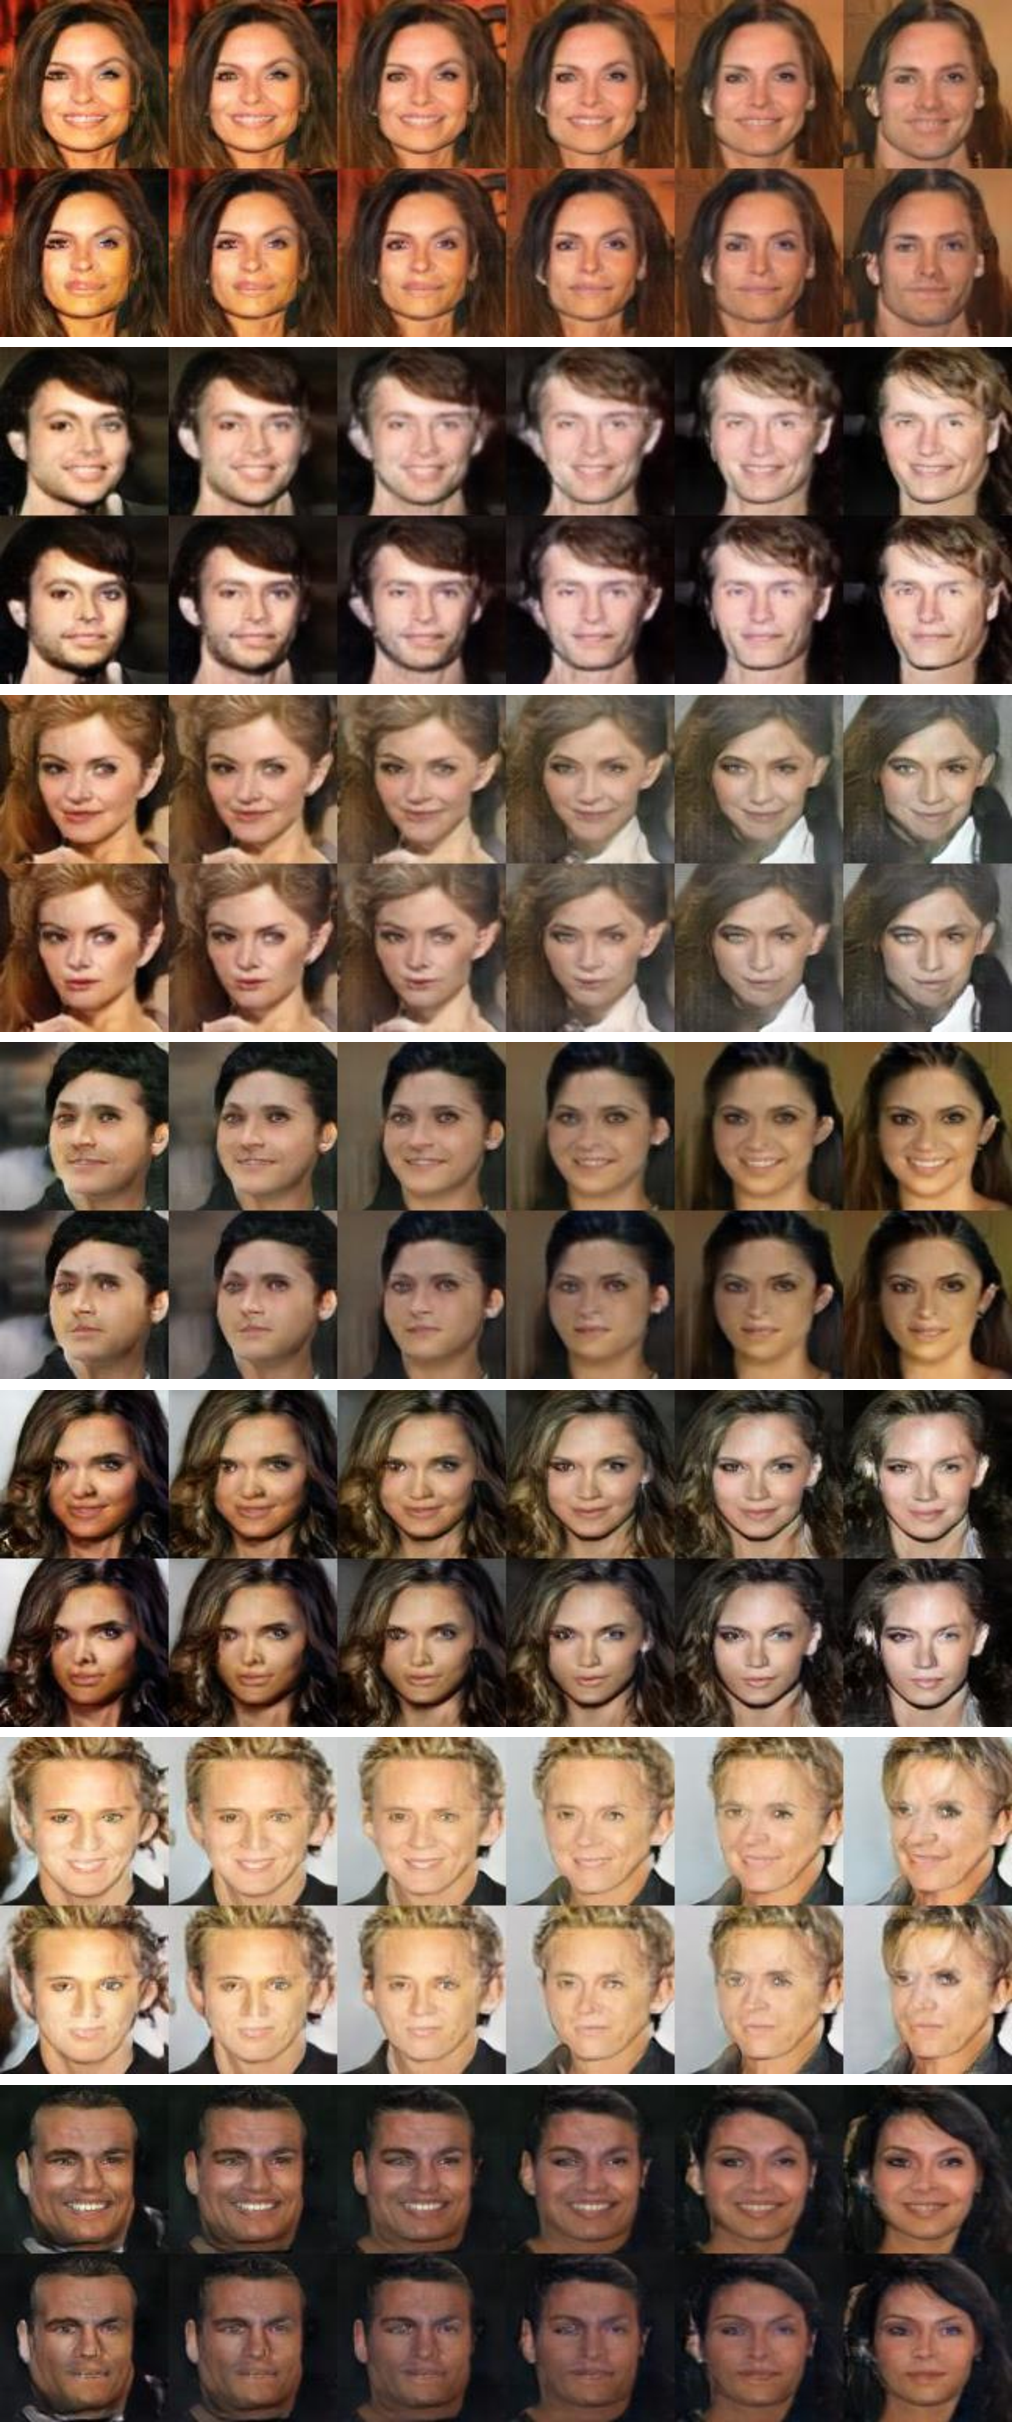
\includegraphics[trim=0in 0in 0in 0in, width=0.65\textwidth]{result_face_smiling_big1.pdf}
\caption{Generation of smiling and non-smiling faces.}
\label{fig::result_smiling1}
\end{figure*}
\begin{figure*}[thb!]
\centering
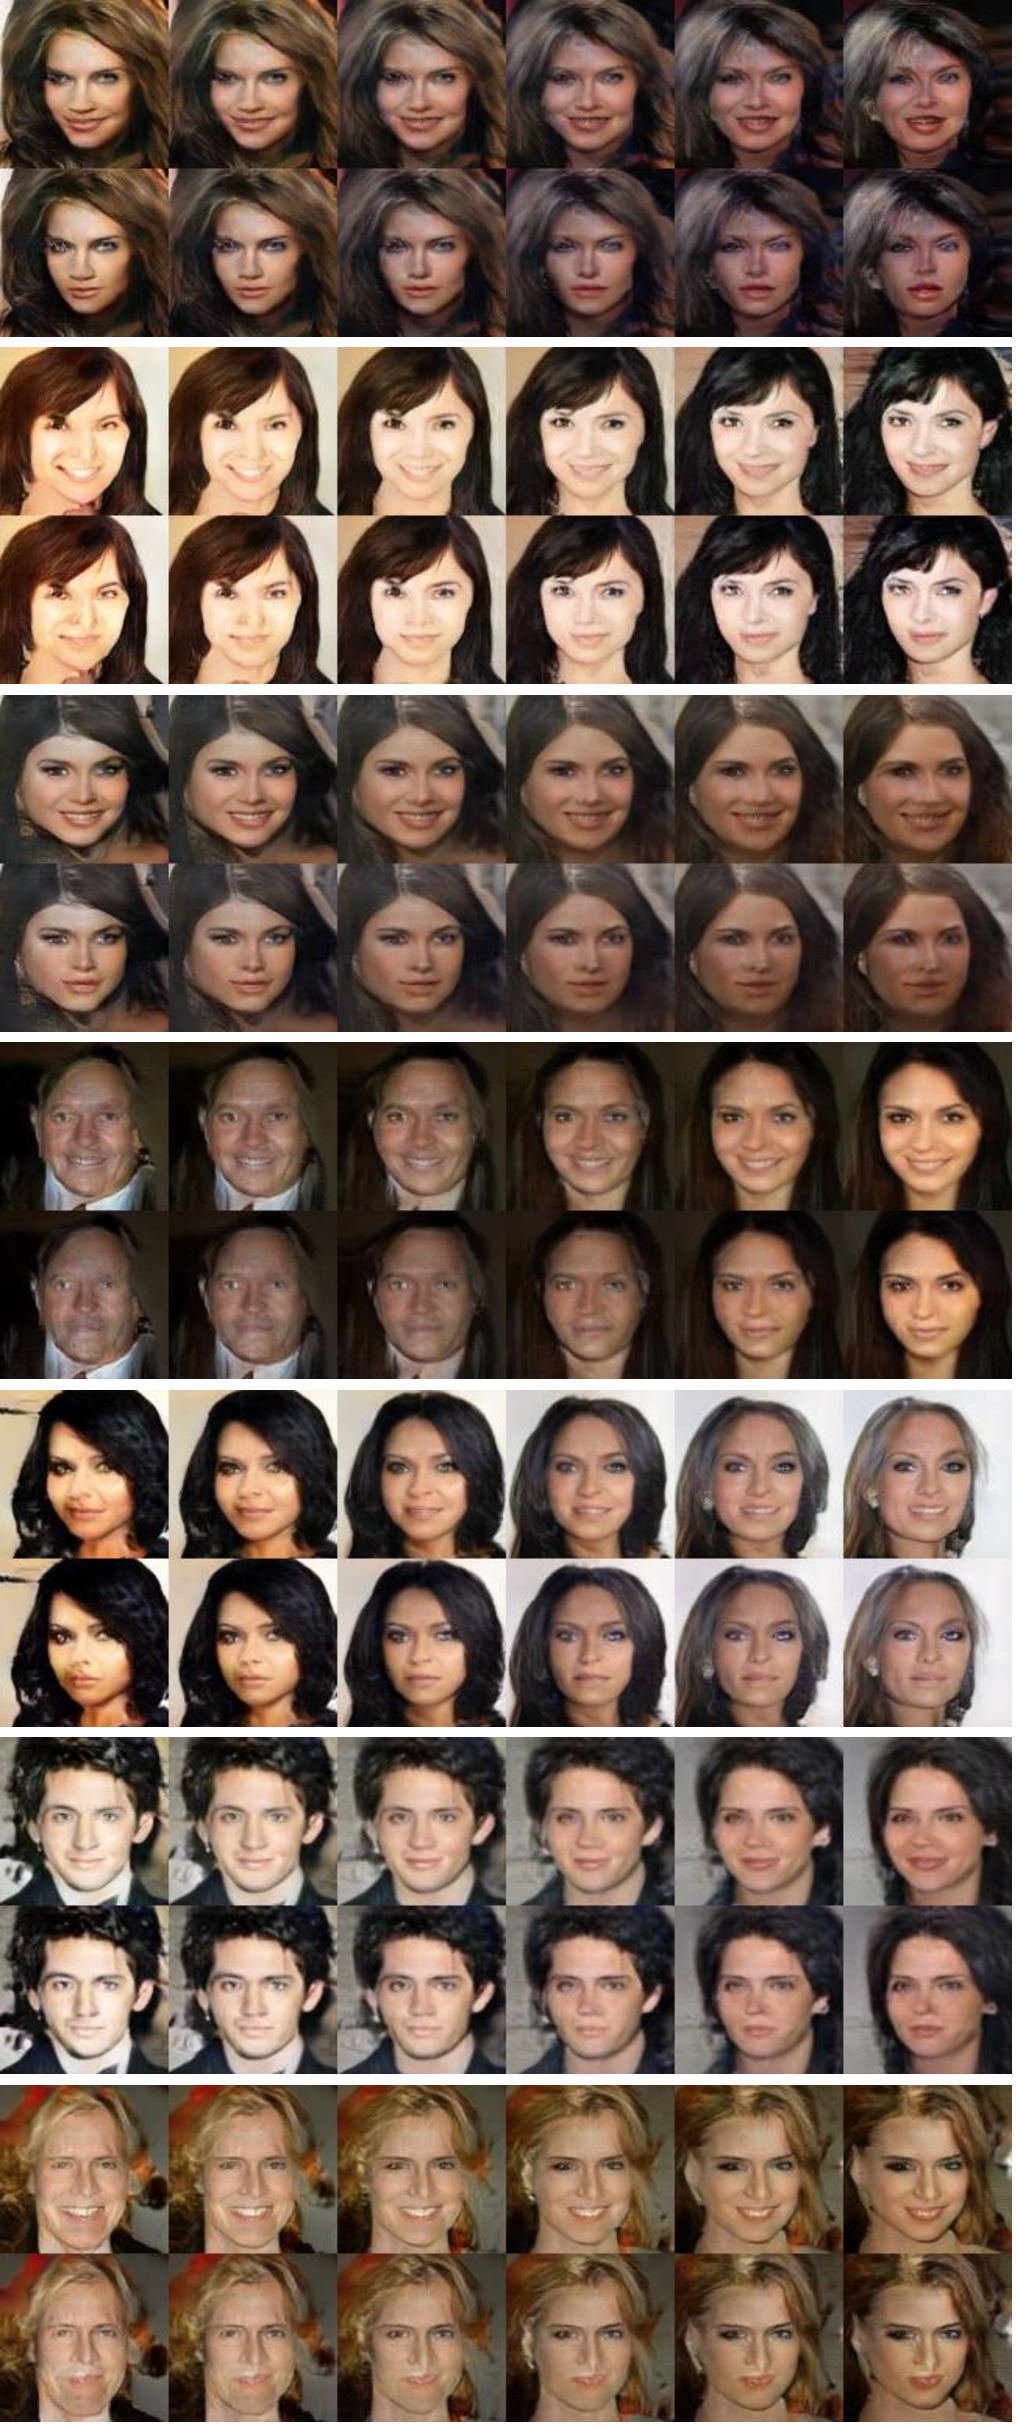
\includegraphics[trim=0in 0in 0in 0in, width=0.65\textwidth]{result_face_smiling_big2.pdf}
\caption{Generation of smiling and non-smiling faces.}
\label{fig::result_smiling2}
\end{figure*}
\begin{figure*}[thb!]
\centering
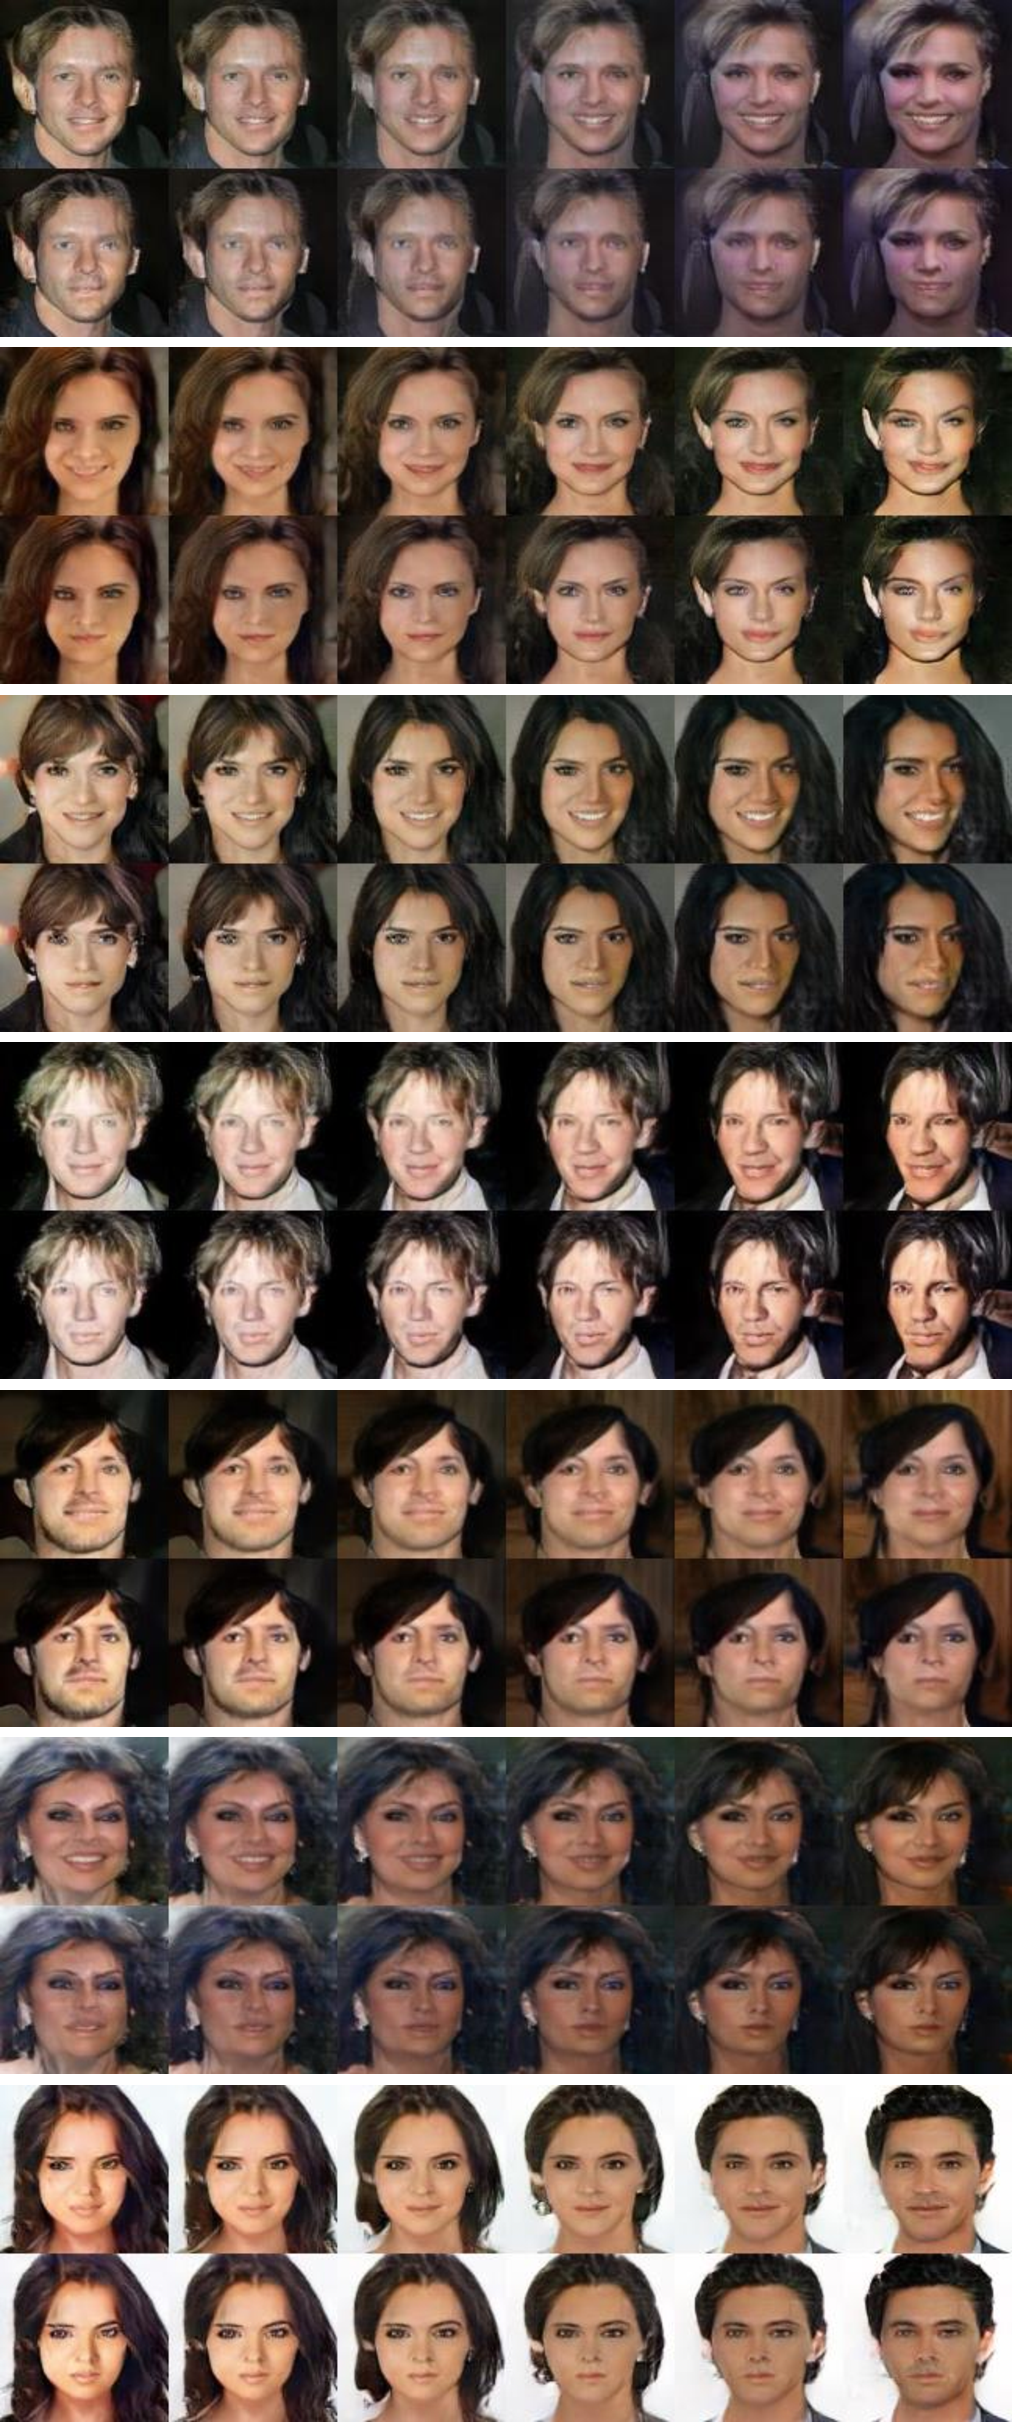
\includegraphics[trim=0in 0in 0in 0in, width=0.65\textwidth]{result_face_smiling_big3.pdf}
\caption{Generation of smiling and non-smiling faces.}
\label{fig::result_smiling3}
\end{figure*}
% %%%%%%%%%%%%%%%%%%%%%%%%%%%%%%%%%%%%%%%%%%%%%%%%%%%%%%%%%%%%%%%%%%%%%%%%%%%%%%%%%%%%%%%%%%%%%%%%%%
\begin{figure*}[thb!]
\centering
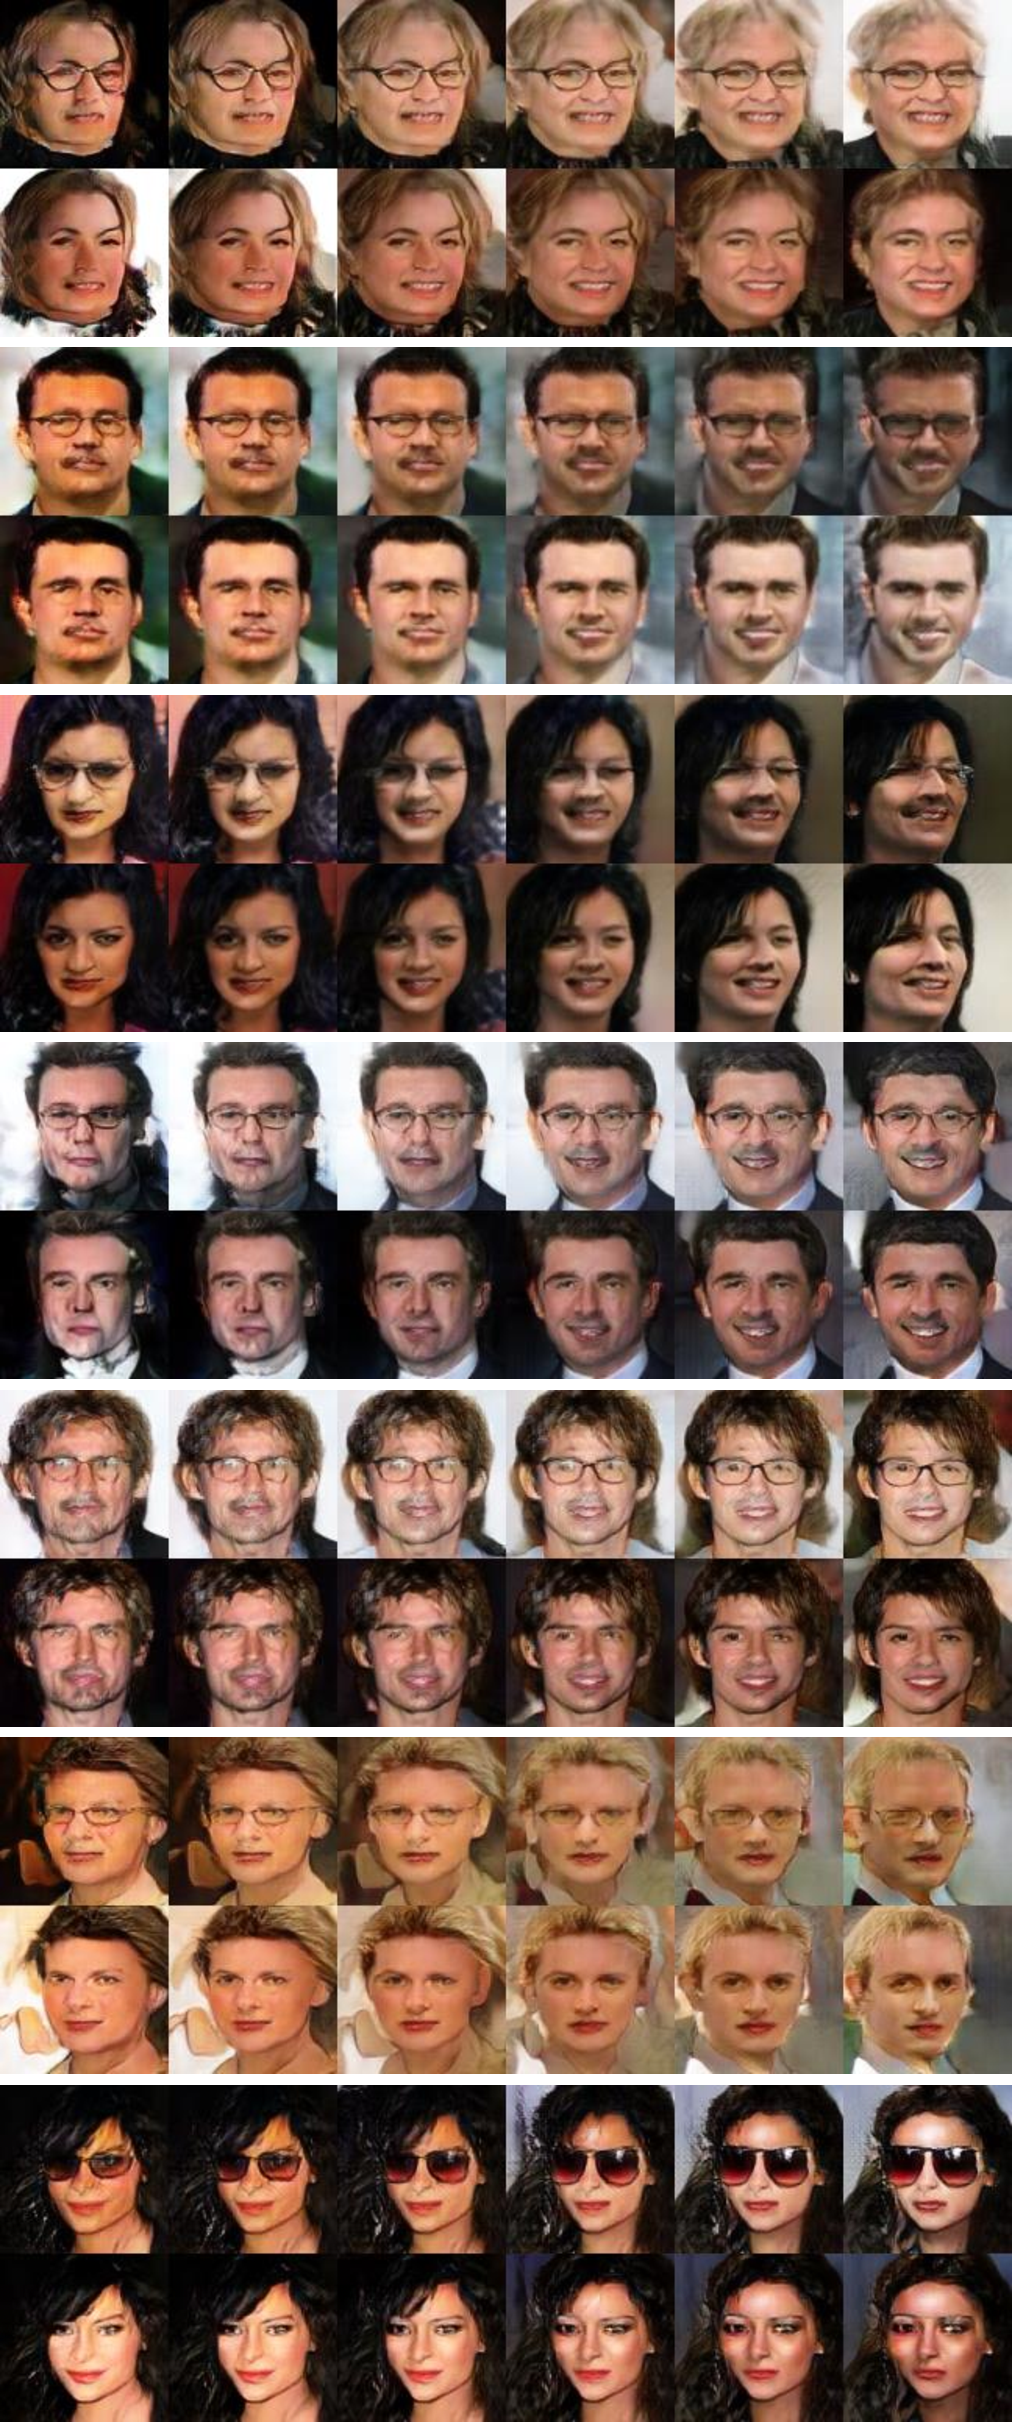
\includegraphics[trim=0in 0in 0in 0in, width=0.65\textwidth]{result_face_eyeglasses_big1.pdf}
\caption{Generation of faces with eyeglasses and without eyeglasses.}
\label{fig::result_eyeglass1}
\end{figure*}
\begin{figure*}[thb!]
\centering
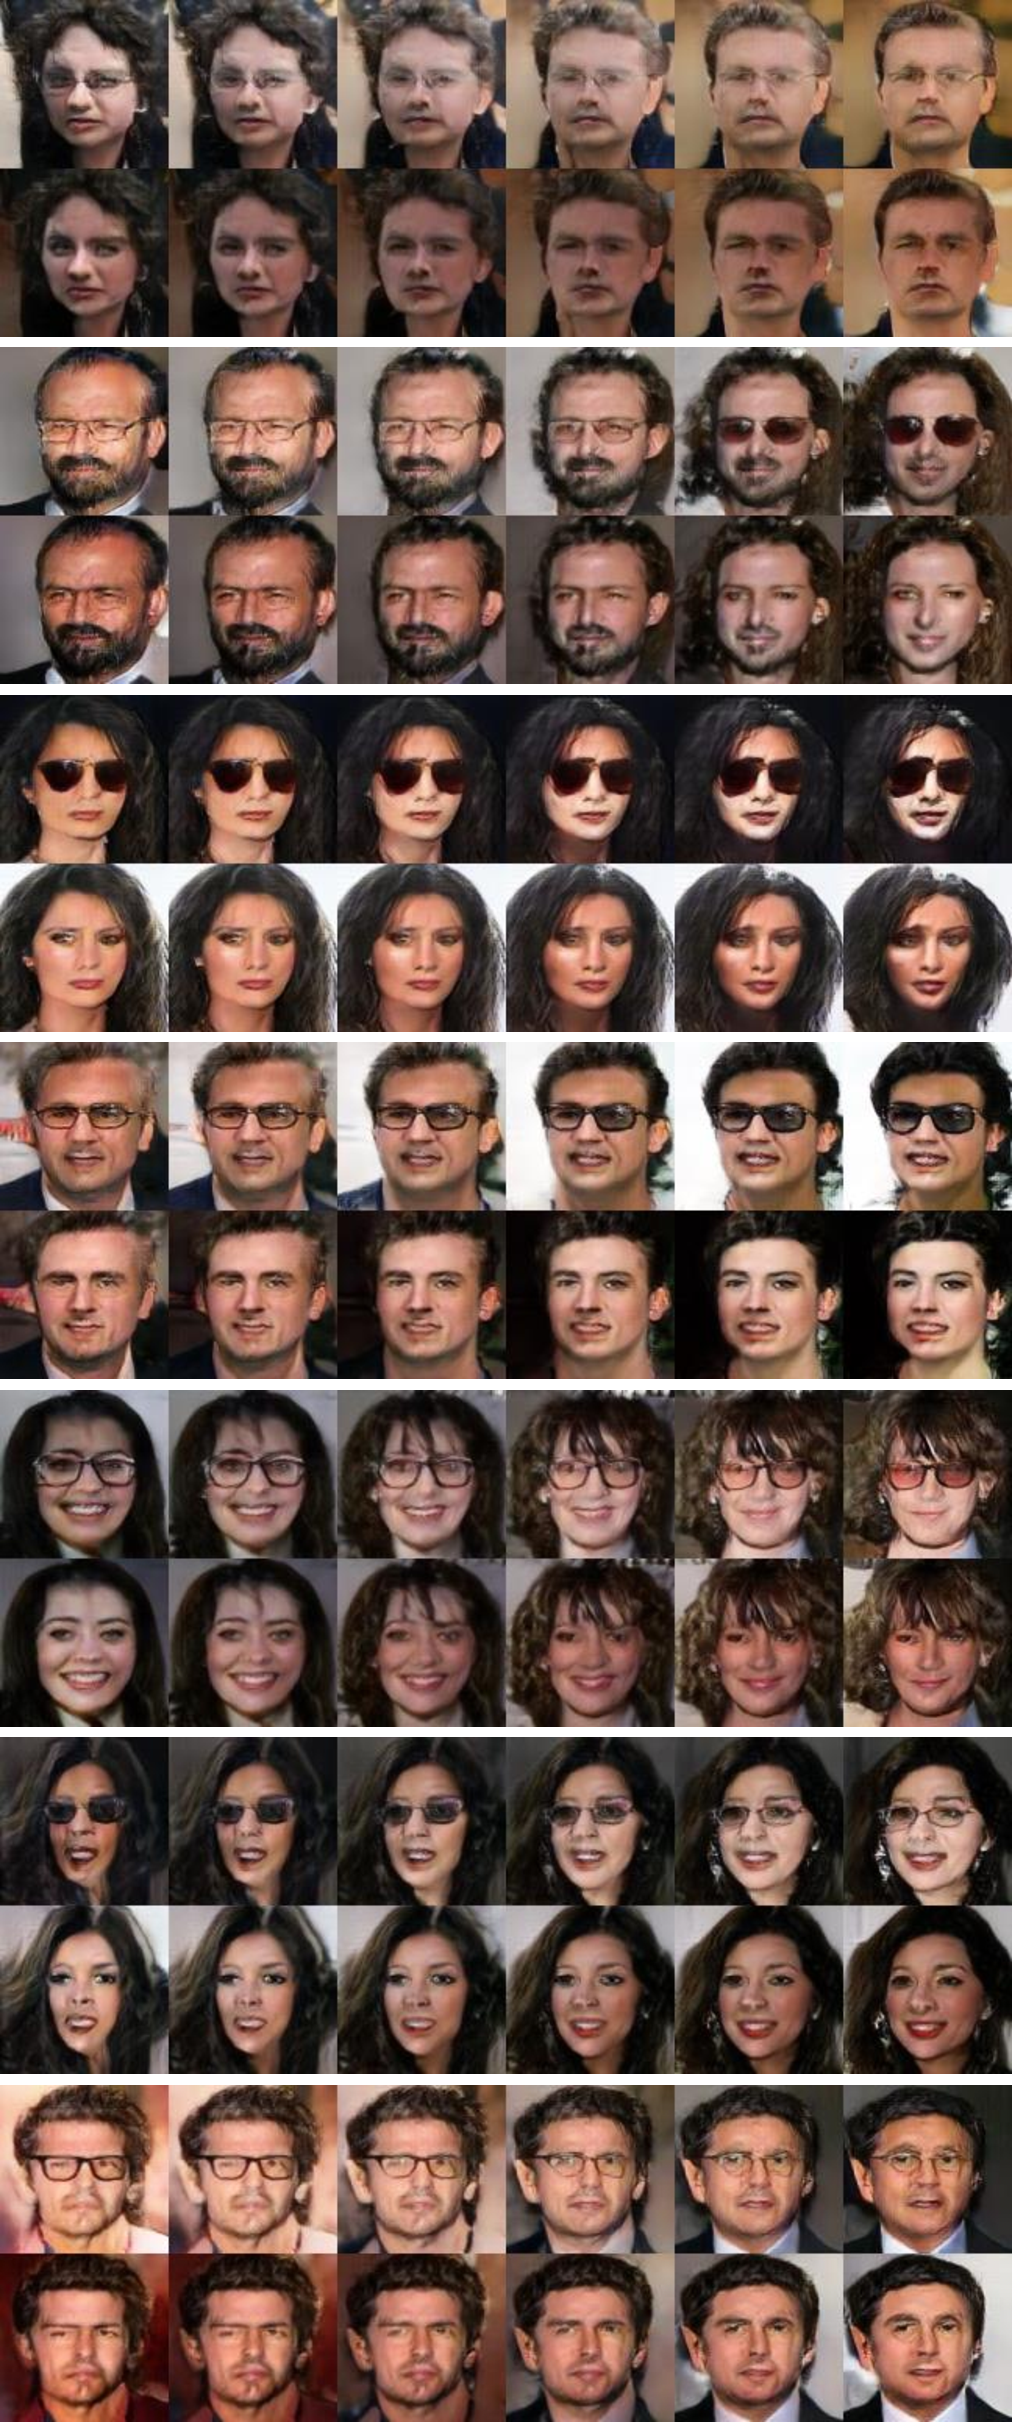
\includegraphics[trim=0in 0in 0in 0in, width=0.65\textwidth]{result_face_eyeglasses_big2.pdf}
\caption{Generation of faces with eyeglasses and without eyeglasses.}
\label{fig::result_eyeglass2}
\end{figure*}
\begin{figure*}[thb!]
\centering
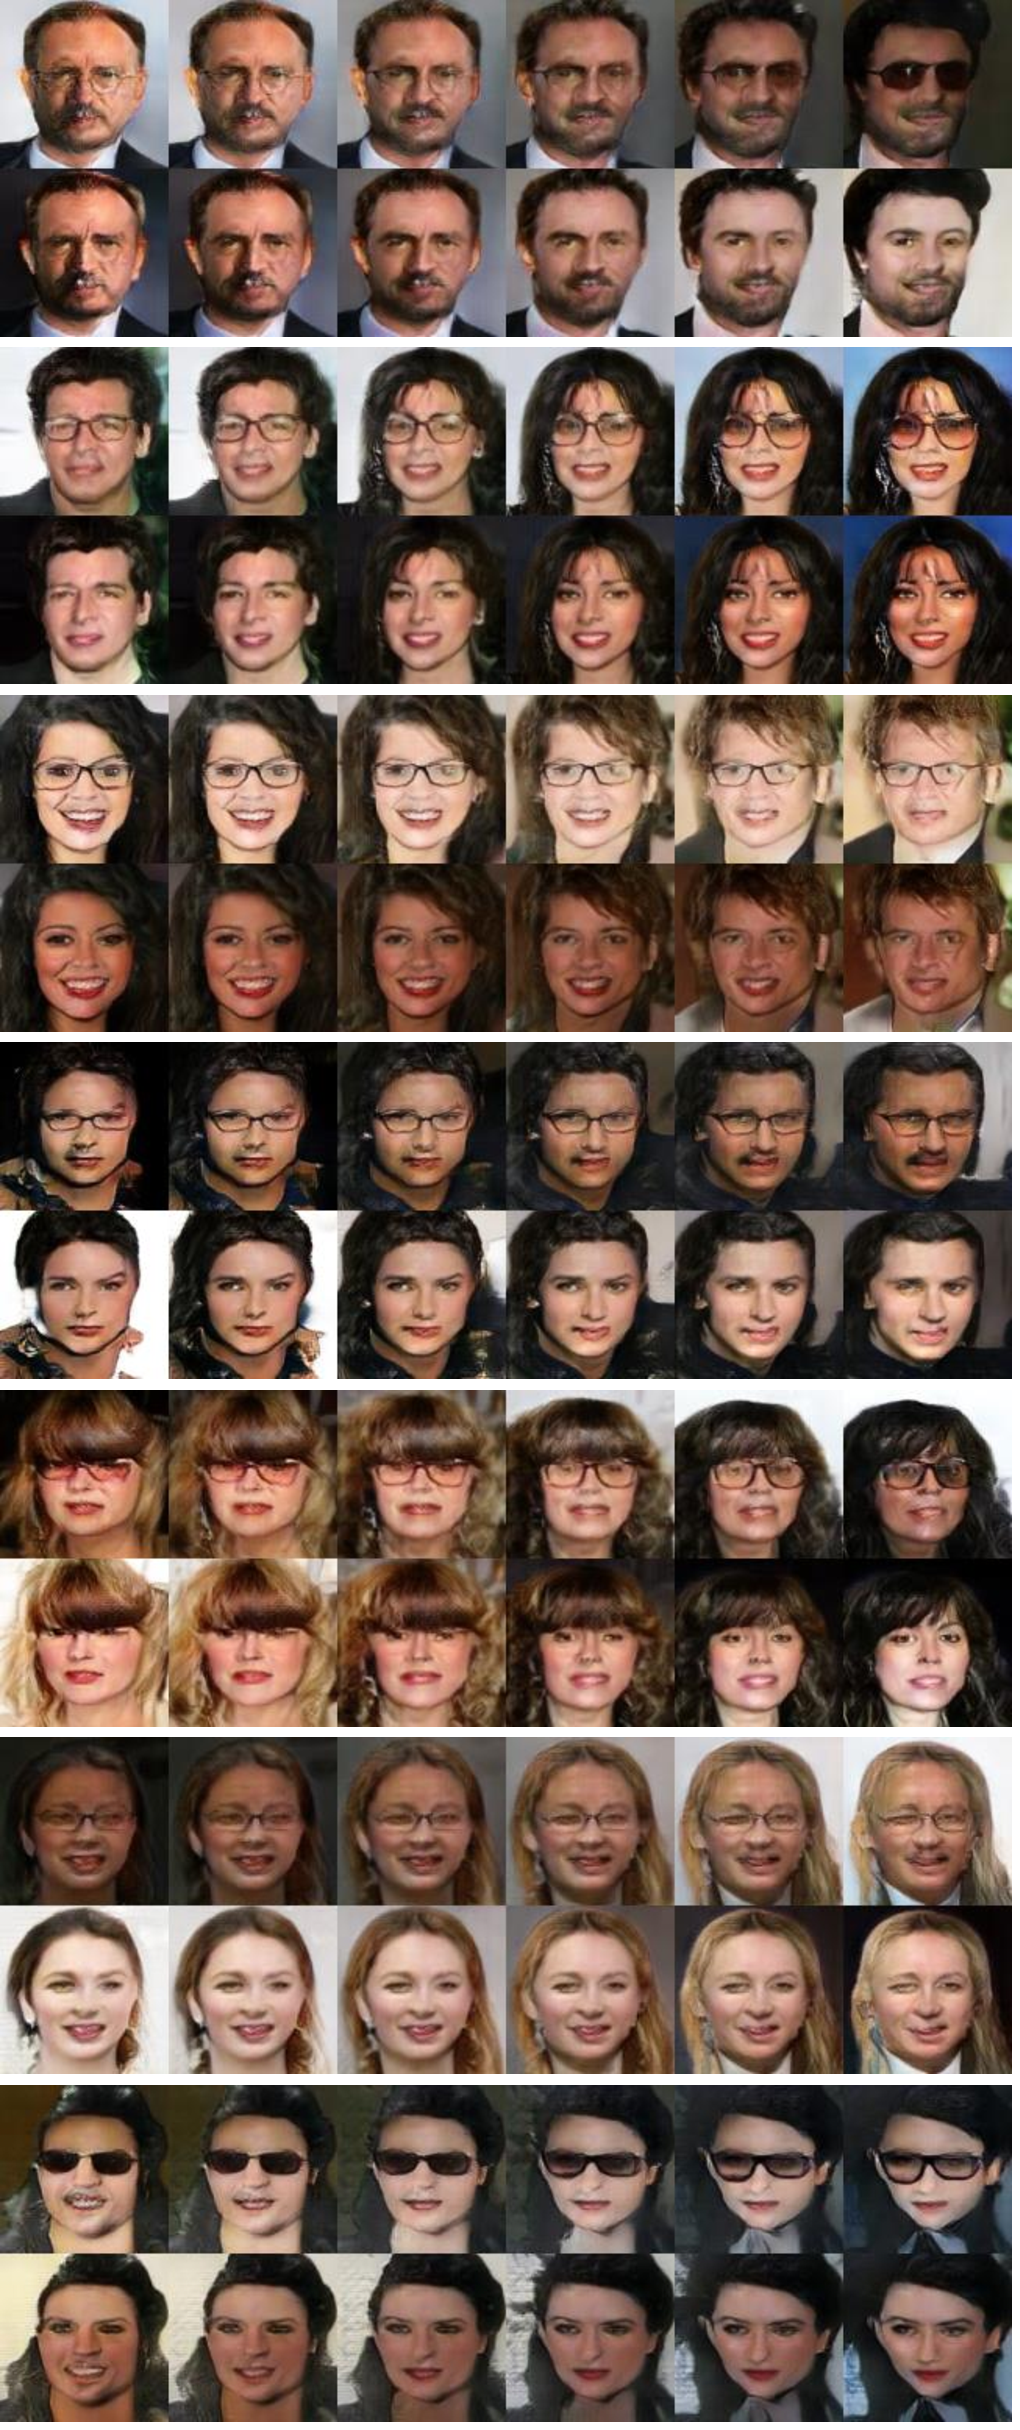
\includegraphics[trim=0in 0in 0in 0in, width=0.65\textwidth]{result_face_eyeglasses_big3.pdf}
\caption{Generation of faces with eyeglasses and without eyeglasses.}
\label{fig::result_eyeglass3}
\end{figure*}

\begin{figure*}[tbh!]
\centering
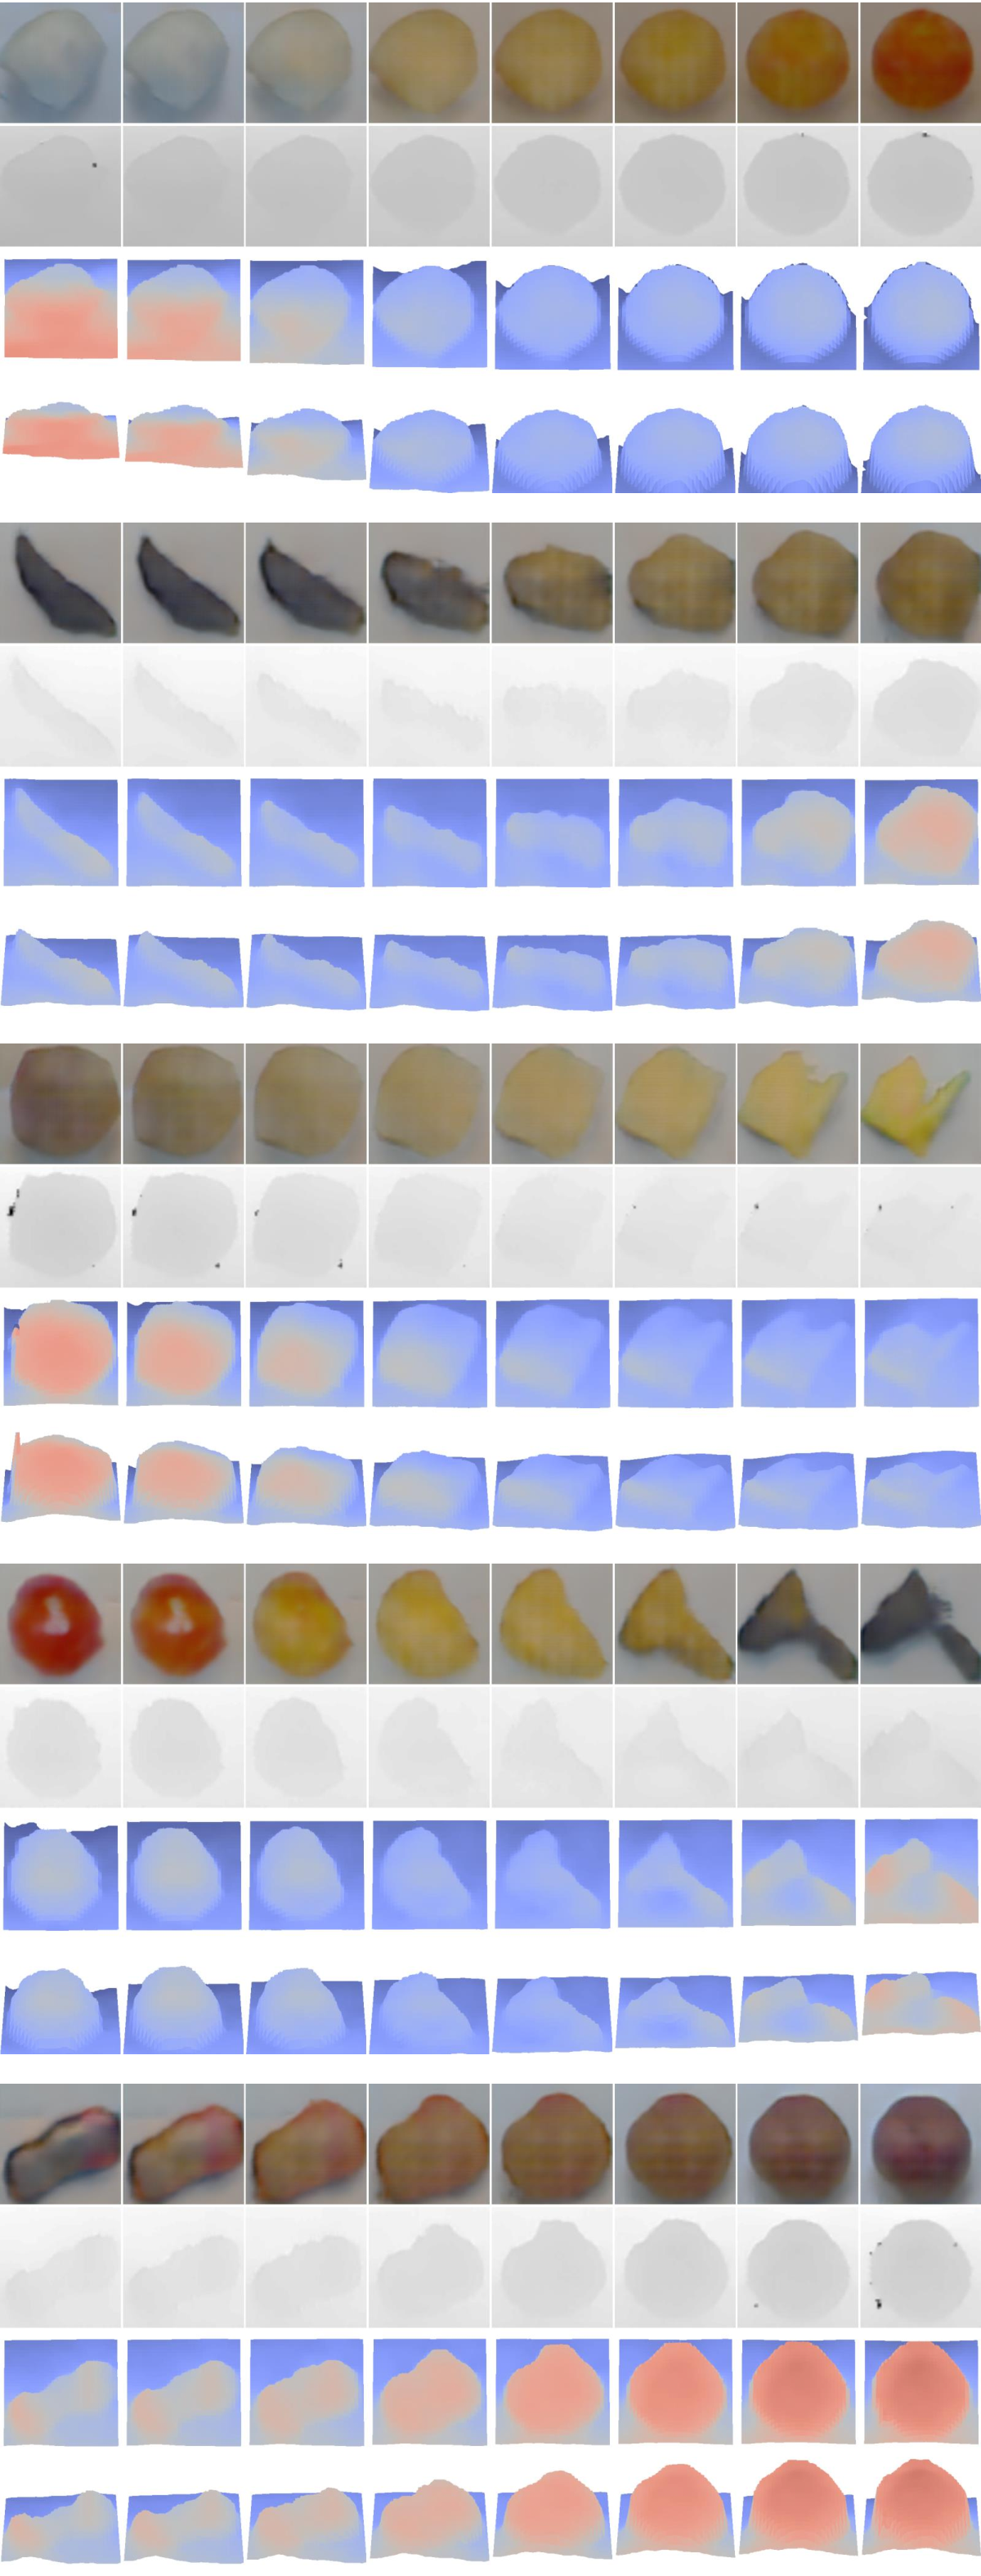
\includegraphics[trim=0in 0in 0in 0in, width=0.57\textwidth]{result_rgbd_big1.pdf}
\caption{Generation of RGB and depth images of objects. The 1st row contains the color images. The 2nd row contains the depth images. The 3rd and 4th rows visualized the point clouds under different view points.}
\label{fig::result_rgbd1}
\end{figure*}

\begin{figure*}[tbh!]
\centering
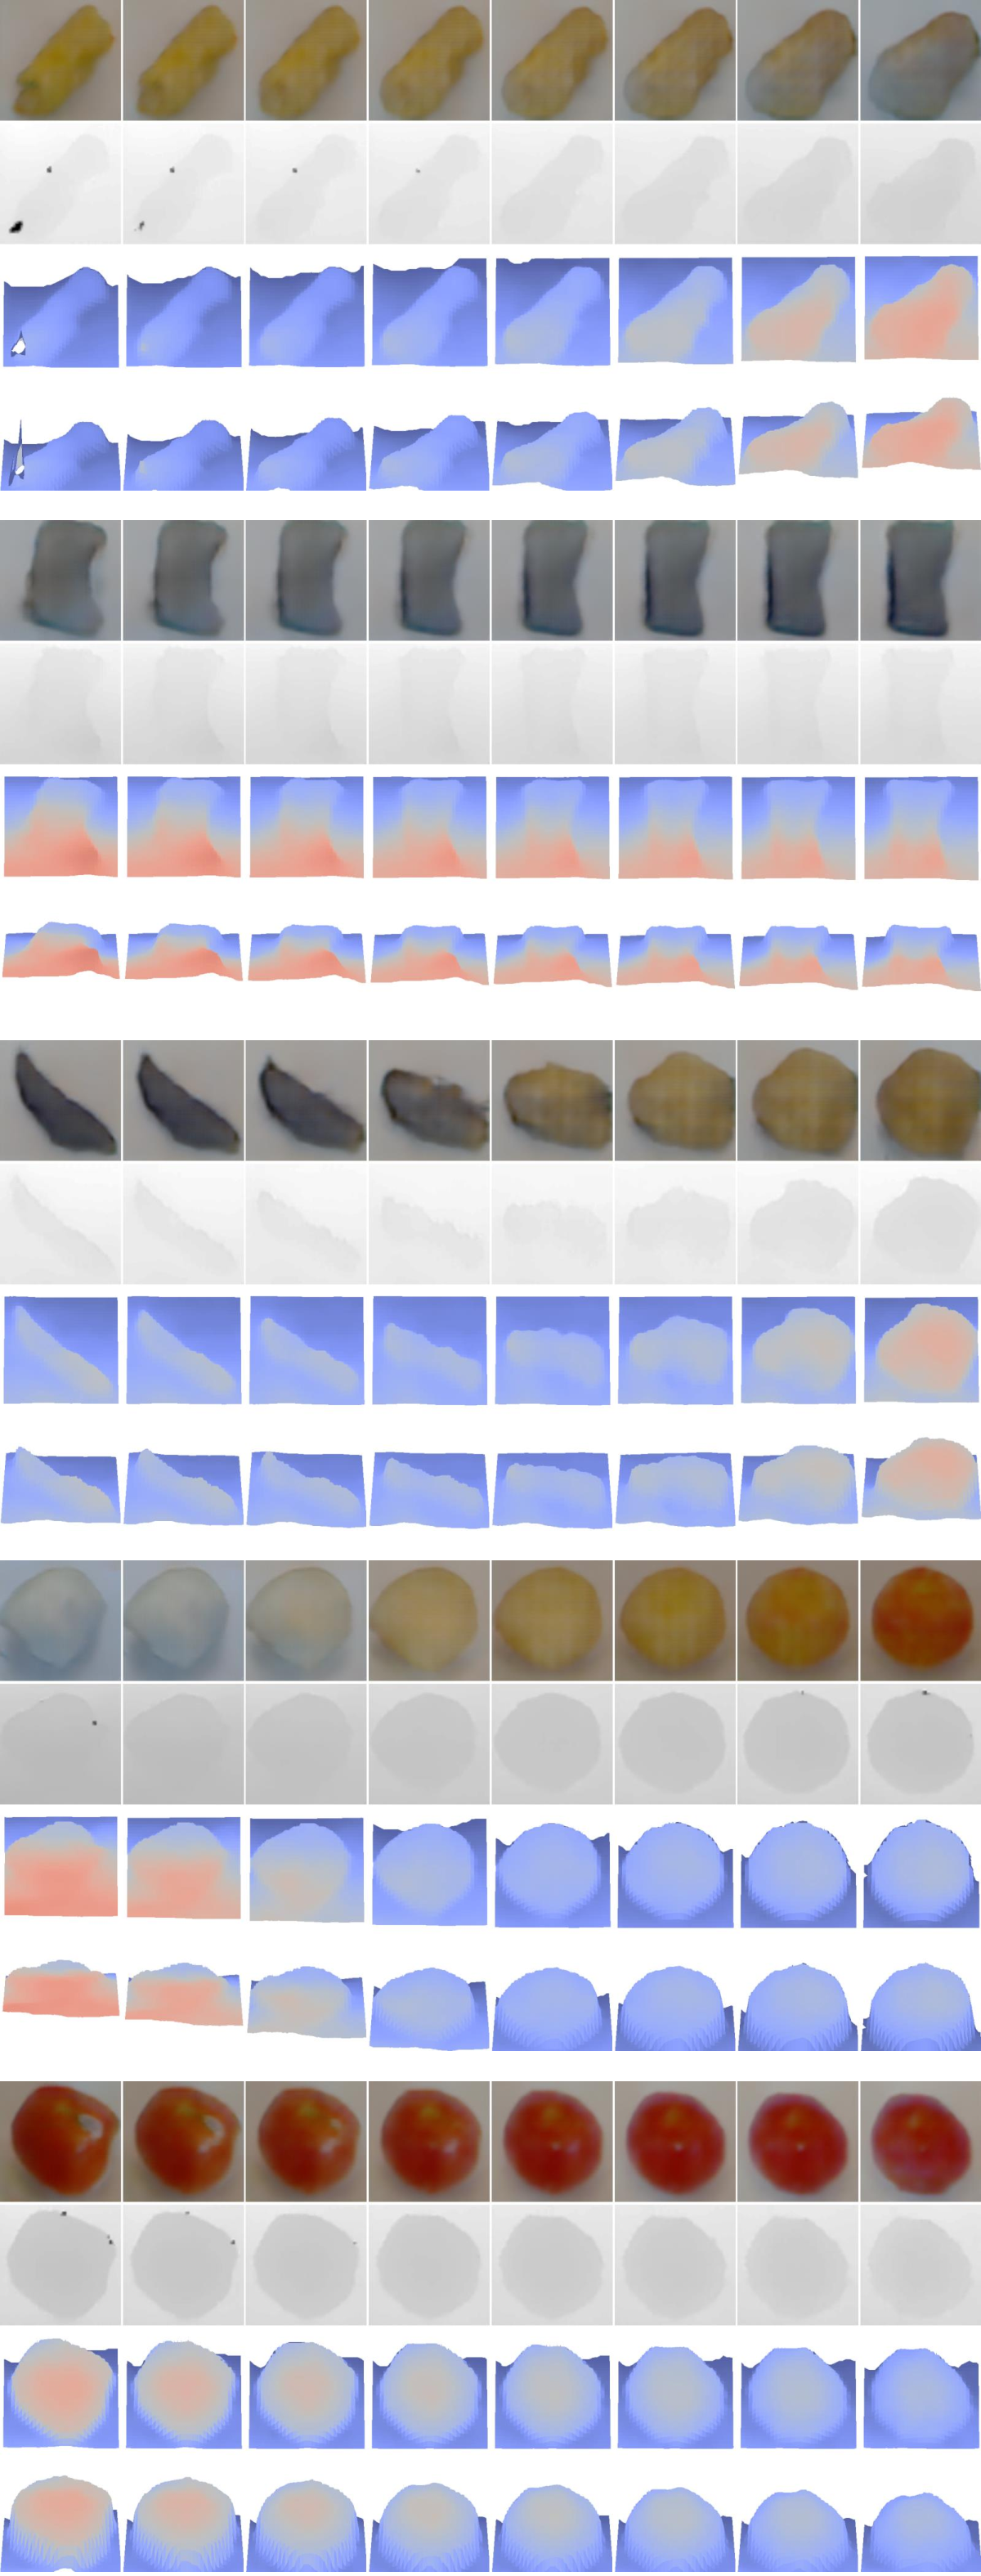
\includegraphics[trim=0in 0in 0in 0in, width=0.57\textwidth]{result_rgbd_big2.pdf}
\caption{Generation of RGB and depth images of objects. The 1st row contains the color images. The 2nd row contains the depth images. The 3rd and 4th rows visualized the point clouds under different view points.}
\label{fig::result_rgbd2}
\end{figure*}

\begin{figure*}[tbh!]
\centering
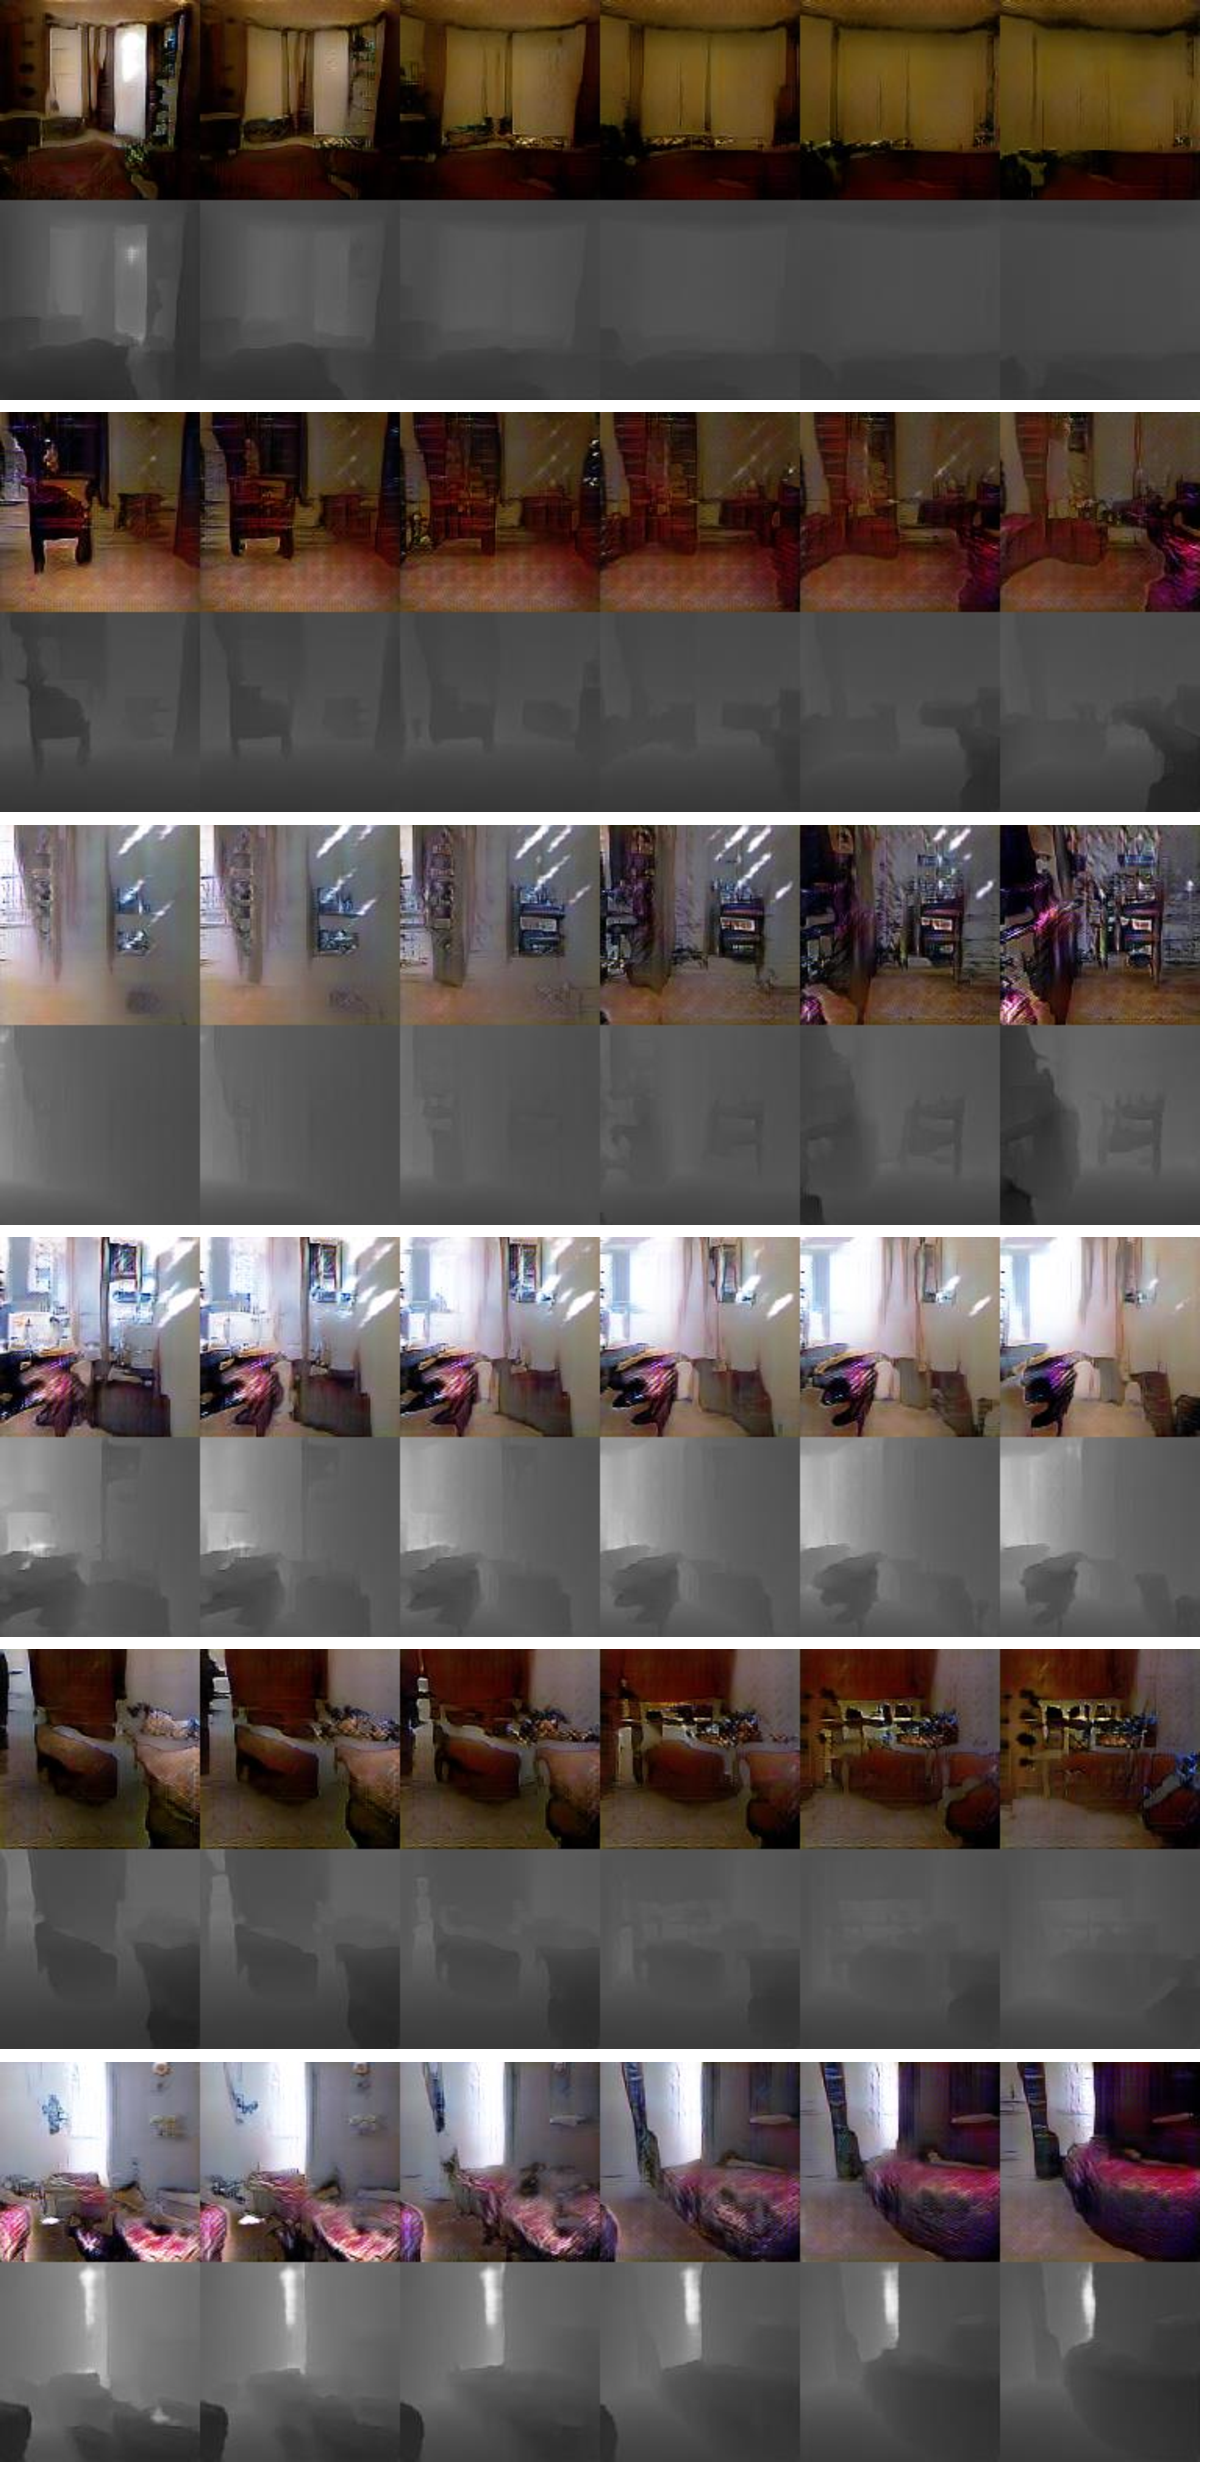
\includegraphics[trim=0in 0in 0in 0in, width=0.75\textwidth]{result_nyu_big1.pdf}
\caption{Generation of RGB and depth images of indoor scenes.}
\label{fig::result_nyu1}
\end{figure*}

\begin{figure*}[tbh!]
\centering
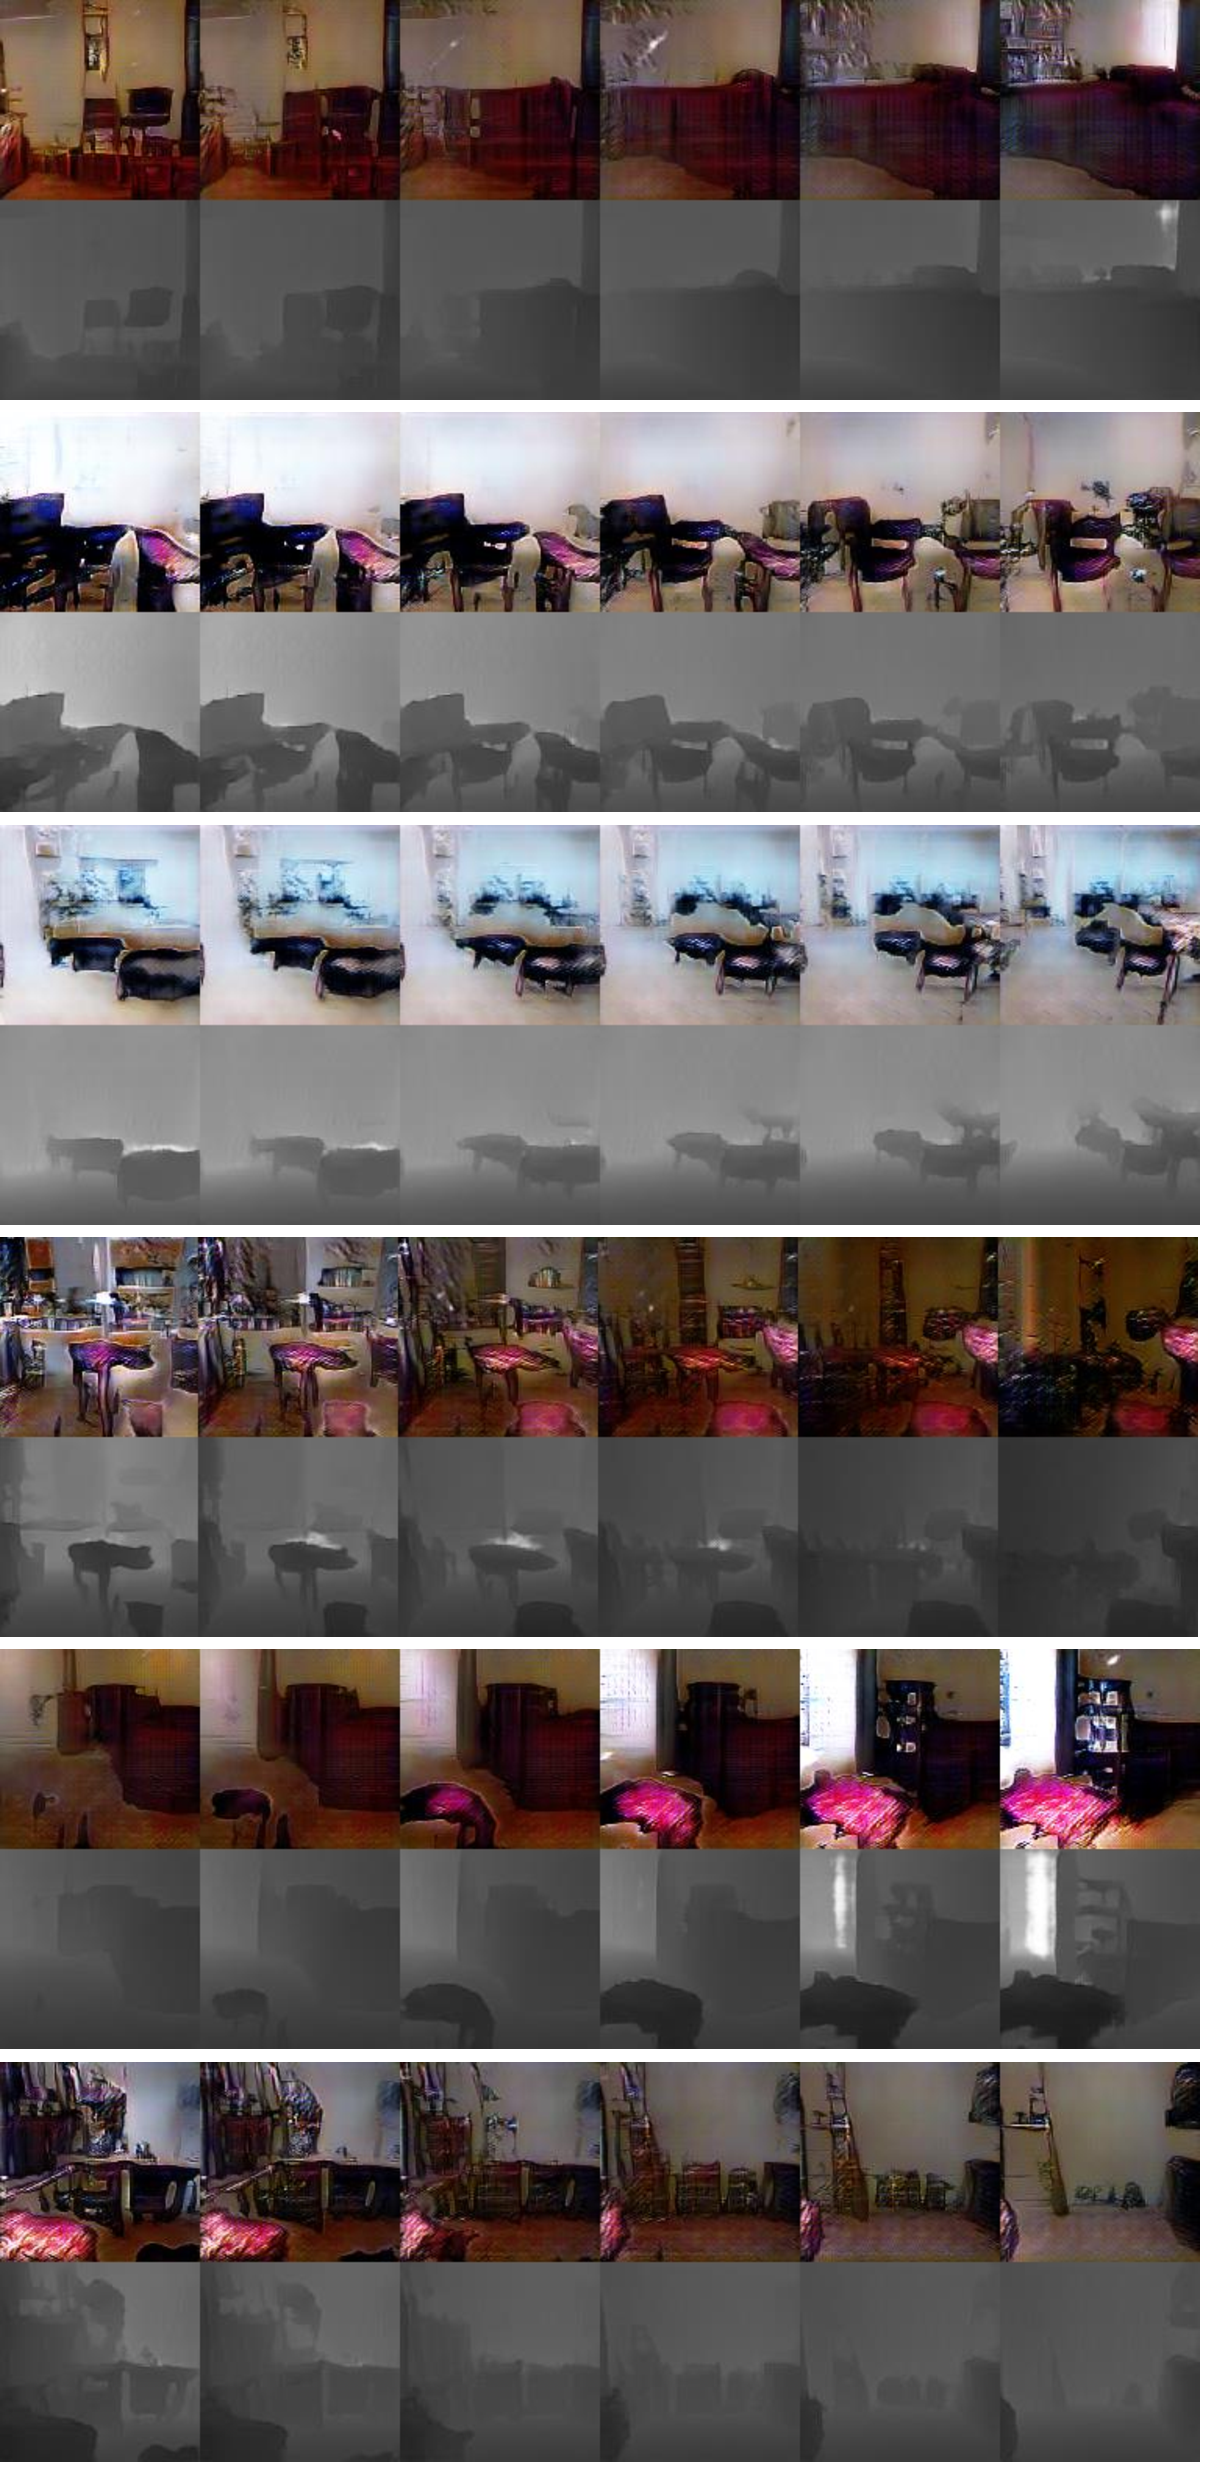
\includegraphics[trim=0in 0in 0in 0in, width=0.75\textwidth]{result_nyu_big2.pdf}
\caption{Generation of RGB and depth images of indoor scenes.}
\label{fig::result_nyu2}
\end{figure*}